\documentclass[a4paper]{article}
% Essential for making this template work are graphicx, float, tabularx, tabu, tocbibind, titlesec, fancyhdr, xcolor and tikz. 

% Not essential, but you will have to debug the document a little bit when removing them are amsmath, amsthm, amssymb, amsfonts, caption, subcaption, appendix, enumitem, hyperref and cleveref.

% inputenc, lipsum, booktabs, geometry and microtype are not required, but nice to have.

% Essential packages
\usepackage[utf8]{inputenc} % Allows the use of some special characters
\usepackage{amsmath, amsthm, amssymb, amsfonts} % Nicer mathematical typesetting
\usepackage{lipsum} % Creates dummy text lorem ipsum to showcase typsetting 
\usepackage{graphicx} % Allows the use of \begin{figure} and \includegraphics
\usepackage{float} % Useful for specifying the location of a figure ([H] for ex.)
\usepackage{caption} % Adds additional customization for (figure) captions
\usepackage{subcaption} % Needed to create sub-figures
\usepackage{tabularx, tabu, booktabs, multirow} % Adds additional customization for tables
\usepackage[nottoc,numbib]{tocbibind} % Automatically adds bibliography to ToC
\usepackage[margin=2.5cm]{geometry} % Allows for custom (wider) margins
\usepackage{titletoc} % Used to create a custom ToC
\usepackage{appendix} % Any chapter after \appendix is given a letter as index
\usepackage{fancyhdr} % Adds customization for headers and footers
\usepackage[shortlabels]{enumitem} % Adds additional customization for itemize 
\usepackage{hyperref} % Allows links and makes references and the ToC clickable
\usepackage[noabbrev, capitalise]{cleveref} % Easier referencing using \cref{<label>} instead of \ref{}
\usepackage{xcolor} % Predefines additional colors and allows user defined colors
\usepackage{tikz} % Useful for drawing images, used for creating the frontpage
\usetikzlibrary{positioning, calc, shapes.geometric, arrows, arrows.meta} % Additional libraries for tikz
\usepackage{chngcntr}
\usepackage{xspace}
\usepackage{longtable}
\usepackage{multirow}
\usepackage{sectsty}
\subsubsectionfont{\normalfont\normalsize\bfseries}
\usepackage{lscape} % hoặc \usepackage{pdflscape} nếu bạn muốn in ra PDF
\usepackage{listings}
\usepackage{microtype}
\usepackage{tocloft}
\usepackage{url}
\usepackage{algorithm}
\usepackage{algpseudocode}
\usepackage{ifxetex}
\usepackage{ifluatex}
\usepackage{vntex}
\usepackage[english]{babel}
\usepackage{fontawesome}
\usepackage{wasysym}
\usepackage{titlesec}
\usepackage{natbib}
% \usepackage{algorithmic}

% Defines a command used by tikz to calculate some coordinates for the front-page
\makeatletter
\newcommand{\gettikzxy}[3]{%
  \tikz@scan@one@point\pgfutil@firstofone#1\relax
  \edef#2{\the\pgf@x}%
  \edef#3{\the\pgf@y}%
}
\makeatother
 % Loads in the preamble 
% Add your group number
\newcommand\groupnumber{
\textbf{Group 07}
}

% Insert authors and student numbers here
\newcommand\reportauthors{
\\
Tran Ly Nhat Hao & 23127187 \\
Pham Thanh Dat & 23127170 \\
Huynh Hao Nam & 23127431 \\
}

% Add the name of your tutor
% \newcommand\grouptutor{
% Tutor: Name Surname
% }

% Date and location
\newcommand\placeanddate{
Ho Chi Minh City, \today
}

% Define Tue-red
\definecolor{Tue-red}{RGB}{199, 25, 24}

% Sets up hyperlinks in the document to be colored
\hypersetup{
    colorlinks=true,
    linkcolor=blue,
    urlcolor=magenta,
    citecolor = Tue-red
}
% \urlstyle{same} % Defines settings for link and reference formatting


% Change bullet style for level 1, 2 and 3 respectively for itemize
% \renewcommand{\labelitemi}{\scriptsize\textcolor{Tue-red}{$\blacksquare$}}% level 1
% \renewcommand{\labelitemii}{\scriptsize\textcolor{Tue-red}{$\square$}}% level 2
% \renewcommand{\labelitemiii}{\textcolor{Tue-red}{$\circ$}}% level 3

% \renewcommand{\labelitemi}{\small\textcolor{Tue-red}{\ding{70}}} % level 1
% \renewcommand{\labelitemii}{\small\textcolor{Tue-red}{\ding{71}}}% level 2
% \renewcommand{\labelitemiii}{\tiny\textcolor{Tue-red}{\ding{71}}}% level 3

% % Change bullet style for level 1, 2 and 3 respectively for enumerate
% \renewcommand{\labelenumi}{\textbf{\textcolor{Tue-red}{\arabic*.}}}% level 1
% \renewcommand{\labelenumii}{\textbf{\textcolor{Tue-red}{[\alph*]}}}% level 2
% \renewcommand{\labelenumiii}{\textbf{\textcolor{Tue-red}{\roman*.}}}% level 3

% Creates a beautiful header/footer
% \lhead{\includegraphics[height = 20pt]{Figures/0. General/us-giraldillo.png}}
% \rhead{\reporttitle}
% \renewcommand{\footrulewidth}{0.4pt}
% \cfoot{Page \thepage}


% Formats section, subsection and subsubsection titles respectively 
% \titleformat{\section}{\sffamily\color{Tue-red}\Large\bfseries}{\thesection\enskip\color{gray}\textbar\enskip}{0cm}{} % Formats section titles

% \titleformat{\subsection}{\sffamily\color{Tue-red}\large\bfseries}{\thesubsection\enskip\color{gray}\textbar\enskip}{0cm}{} % Formats subsection titles

% \titleformat{\subsubsection}{\sffamily\color{Tue-red}\bfseries}{\thesubsubsection\enskip\color{gray}\textbar\enskip}{0cm}{} % Formats subsubsection titles

% Formats captions
% \DeclareCaptionFont{Tue-red}{\color{Tue-red}}
% \captionsetup{labelfont={Tue-red,bf}}

\titleformat{\subsection}
{\normalfont\Large\bfseries}{\thesubsection}{1em}{}

\titleformat{\section}
{\normalfont\Large\bfseries}{\thesection}{1em}{}

\counterwithin{figure}{section}  % Number figures by section
\counterwithin{table}{section}   % Number tables by section
\renewcommand{\thefigure}{\thesection.\arabic{figure}}  % Format figure numbering
\renewcommand{\thetable}{\thesection.\arabic{table}}    % Format table numbering
\renewcommand{\refname}{\Large References}
\renewcommand{\labelitemi}{$\bullet$}


% ============ CODE ============
\usepackage{listings}
\usepackage{xcolor}
\definecolor{codegreen}{rgb}{0,0.6,0}
\definecolor{codegray}{rgb}{0.5,0.5,0.5}
\definecolor{codepurple}{rgb}{0.58,0,0.82}
\definecolor{backcolour}{rgb}{0.95,0.95,0.92}

% Styling for the code.
\lstdefinestyle{mystyle}{
    backgroundcolor=\color{backcolour},   
    commentstyle=\color{codegreen},
    keywordstyle=\color{magenta},
    numberstyle=\tiny\color{codegray},
    stringstyle=\color{codepurple},
    basicstyle=\ttfamily\footnotesize,
    breakatwhitespace=false,         
    breaklines=true,                 
    captionpos=b,                    
    keepspaces=true,                 
    numbers=left,                    
    numbersep=5pt,                  
    showspaces=false,                
    showstringspaces=false,
    showtabs=false,                  
    tabsize=2
}

\lstdefinestyle{pythonstyle}{
    language=Python,
    basicstyle=\ttfamily\small,
    commentstyle=\color{green!40!black},
    keywordstyle=\color{blue},
    numberstyle=\tiny\color{gray},
    numbers=left,
    stepnumber=1,
    frame=single,
    breaklines=true,
    breakatwhitespace=false,
    tabsize=4,
    showstringspaces=false,
    captionpos=b,
    morekeywords={True, False},
}

\lstset{style=mystyle}

% Disable indentation on new paragraphs
\setlength{\parindent}{0pt}

\newcommand{\coursename}{Data Structures and Algorithms}
\newcommand{\reportname}{Algorithm survey and evaluation}
\newcommand{\reporttitle}{Sorting Algorithms}

% \newcommand{\studentname}{ \\ }
\newcommand{\teachername}{%
  \makebox[4.0cm][l]{MSc. Phan Thi Phuong Uyen}%
  \\
  \makebox[4.0cm][l]{TA. Tran Hoang Quan}%
}
\newcommand{\leftfooter}{\LaTeX\ by \href{https://github.com/tranlynhathao}{tranlynhathao}}


% ============ HEADER AND FOOTER ============
% Header length
\setlength{\headheight}{29.43912pt}

% Footer page number would be on the lower-right corner
\pagestyle{fancy}
\fancyfoot{}
\fancyfoot[R]{Page \thepage}
\renewcommand{\footrulewidth}{1pt}
\renewcommand{\headrulewidth}{1pt}

\lhead{\protect\reporttitle}

\rhead{
University of Science - VNU HCMC\\
\coursename
}
\lfoot{\leftfooter} % Loads in user defined settings

% ============ DOCUMENT ============
\begin{document}
\pagenumbering{arabic}
\setcounter{page}{1} 
% Inserts the front page
\begin{titlepage}

\centering

\begin{center}
\begin{tikzpicture}[remember picture, overlay]
    % VNU logo
    \node[opacity=0.2,inner sep=0pt] at (0, 0) {
\includegraphics[width=1\textwidth]{Figures/0. General/VNU_gray.png}};
    
    % HCMUS logo
    \node[inner sep=0pt] (logo) at (-3, 0) {
\includegraphics[width=.55\textwidth]{Figures/0. General/hcmus.png}};
    
    % FIT
    \node[text width=0.5\textwidth, right=of logo] (title) {
\includegraphics[width=.6\textwidth]{Figures/0. General/fit.png}};
    
    % Red line
    \draw[line width=1mm, Tue-red] ($(logo.east) + (0.5, 1.3)$) -- ($(logo.east) + (0.5, -1.3)$);
\end{tikzpicture}
\end{center}

\vspace{3cm}
\newcommand{\HRule}{\rule{\linewidth}{0.5mm}}
\HRule \\[0.4cm]
{ 
\huge{\bfseries{\reporttitle}}\\[0.5cm]
\large{\bfseries{Topic: \reportname}}
}\\[0.4cm]
\HRule \\[0.7cm]

\textbf{\large Course: \coursename}\\[0.7cm]

\begin{minipage}[t]{0.4\textwidth}
\begin{flushleft} \large
% \emph{Students execute:}\\
% \studentname
\end{flushleft}
\end{minipage}
~
\begin{minipage}[t]{0.4\textwidth}
\begin{flushright} \large
\emph{Supervisor:} \\
\teachername
\end{flushright}
\end{minipage}\\[1cm]

\large \sffamily\groupnumber

\begin{table}[H]
    \centering
    \large
    \begin{tabu} to 0.8\linewidth {cc}
        \sffamily \textbf{Full Name} & \sffamily \textbf{Student ID}\\
        \hline
        \reportauthors
    \end{tabu}
\end{table}


% \sffamily \grouptutor

\tikz[remember picture,overlay]\node[anchor=south,inner sep=0pt] at (current page.south) {
\includegraphics[width=\paperwidth]{Figures/0. General/fixed.jpeg}};

\mbox{}
\vfill
% \sffamily 
\Large \textcolor{white}{\normalfont \placeanddate} \\

\end{titlepage}









\newpage

% Table of Contents
\tableofcontents
\newpage

\phantomsection
\listoffigures
\newpage

% \input{Contents/0. Student_info}
% \newpage

% \section{Introduction}

This report is prepared for the Data Structures and Algorithms project by group 07 under the supervision of MSc. Phan Thi Phuong Uyen and TA. Tran Hoang Quan.

\vspace{10pt}

The aim of this report is to provide a comprehensive survey and evaluation of  the running time and the number of comparisons of various sorting algorithms, highlighting their core concepts, step-by-step explanations, complexity analyses, and possible optimizations.

\vspace{10pt}

Sorting algorithms are fundamental to computer science, playing a critical role in data organization, searching efficiency, and overall computational performance. Understanding these algorithm is essential for solving the problems efficiently.

\vspace{10pt}

This report covers an extensive range of sorting algorithms including Selection Sort, Insertion Sort, Shell Sort, Bubble Sort, Heap Sort, Merge Sort, Quick Sort, Radix Sort, Counting Sort, Binary Insertion Sort, Shaker Sort, and Flash Sort. Each algorithm is discussed in terms of its core concepts, detailed explanations, complexity analyses, and any notable variants or optimizations. The report also encompasses a comprehensive survey and evaluation of the mentioned sorting algorithms focusing on the time of their performance and their number of comparisons.

% \newpage

% % content
% \section{Sorting Algorithms}
% \subsection{Selection Sort}

\subsubsection{Core concept}
Selection sort is comparison-based sorting algorithm. The algorithm repeatedly selects the smallest (or largest) element from the unsorted portion of the list and swaps it with the first element of the unsorted part. This process is repeated for the remaining unsorted portion until the entire list is sorted. ~\cite{ref6}

\vspace{5pt}

\subsubsection{Explanation}
\textbf{One way to explain the algorithm:} ~\cite{ref7}
\begin{itemize}
    \item \textbf{Initialization:} Start with the first element in the list (index 0) as the current minimum.
    \item \textbf{Find the Maximum:} Traverse the unsorted part of the list to find the maximum element.
    \item \textbf{Swap:} Swap the found maximum element with the first element of the unsorted part.
    \item \textbf{Move the Boundary:} Move the boundary between the sorted and unsorted parts one element to the left.
    \item \textbf{Repeat:} Repeat for the next position in the list until the entire list is sorted.
\end{itemize}

\vspace{10pt}

\textbf{Step-by-step:}
\begin{itemize}[label=-]
    \item Consider the following array as an example: { 29, 10, 14, 37, 13}

    \item Beginning with five integers as unsorted part, you select the largest which is 37 and swap it with the last integer 13, then 37 is now in sorted part.

    \item After first swap: {29, 10, 14, 13, 37}

    \item Next you select the largest integer 29 from among the first four integers in the array and swap it with the next-to-last integer in the array 13. 29 is now the first element of sorted part.

    \item After second swap: {13, 10, 14, 29, 37}

    \item Notice that 14 is the largest element in unsorted part and it also is in the proper position in sorted part, but the algorithm ignores this fact and performs a swap of 14 with itself.

    \item After third swap: {13, 10, 14, 29, 37}

    \item Finally, select the 13 and swap it with the item in the second position of the array—10.

    \item After fourth swap: {10, 13, 14, 29, 37}

    \item The array is now sorted into ascending order.
\end{itemize}

\vspace{5pt}

\subsubsection{Complexity analysis}

\textbf{Time complexity:}
At each iteration, the array is divided into two subarrays, the left part is sorted, and the right part is unsorted.

\textbf{Iteration 1:} Perform $n - 1$ comparisons in $n$ numbers, choose the smallest element to move to $a[0]$

\textbf{Iteration 2:} Perform $n - 2$ comparisons in $(n - 1)$ numbers, choose the smallest element to move to $a[1]$

...

\textbf{Iteration $n - 1$:} Perform 1 comparison in 2 numbers $a[n - 2]$ and $a[n - 1]$, choose the smallest element to move to $a[n - 1]$, then $a[n - 1]$ becomes the largest number, ending the algorithm.

Let $f(n)$ be the cost function of the algorithm. We have:

\[
f(n) = (n - 1) + (n - 2) + \ldots + 3 + 2 + 1 = \frac{n(n - 1)}{2} \in O(n^2)
\]
\begin{itemize}
    \item \textbf{Best Case:} $O(n^2)$ – Selection sort always performs $O(n^2)$ comparisons and swaps regardless of the initial order of the elements.
    \item \textbf{Average Case:} $O(n^2)$ – Same as the best case, selection sort does not change its behavior based on the input data.
    \item \textbf{Worst Case:} $O(n^2)$ – Selection sort performs $O(n^2)$ comparisons and swaps in all cases.
\end{itemize}

\textbf{Space complexity:}
\begin{itemize}
    \item $O(1)$ – Selection sort is an in-place sorting algorithm, meaning it requires only a constant amount of additional memory space.
\end{itemize}

\subsubsection{Variants and optimizations}

An optimized variant is heap sort which we will discuss it later. This sorting algorithm is an improvement of selection sort. Heap sort reduces the time to find the smallest or largest element in unsorted part by building a max heap or min heap. Heap is a data structure which is used to find the minimum (min heap) or maximum (max heap) element more efficiently. This reduces the time complexity to $O(n\log n)$.

\vspace{10pt}
% \subsection{Insertion Sort}

\subsubsection{Core Concepts}
Insertion sort orders a list of values by repetitively inserting a particular value into a sorted subset of the list. More specifically, consider the first item to be a sorted sublist of length 1, insert second item into sorted sublist, shifting first item if needed. Insert third item into sorted sublist, shifting items 1-2 as needed. Repeat until all values have been inserted into proper positions. ~\cite{ref1}

\vspace{5pt}

\subsubsection{Step-by-step Explaination}
\begin{itemize}[label=-]
    \item Step 1: Assume the first element is already sorted. Pick the next element and find its correct position among the already sorted elements.
    \item Step 2: Shift all the elements greater than the picked element to one position ahead to make space for the picked element.
    \item Step 3: Insert the picked element into its correct position.
    \item Step 4: Repeat the above steps for all elements in the array.
\end{itemize}

\subsubsection{Complexity Analysis:}
At each iteration, the array is divided into two subarrays, the left part is sorted, and the right part is unsorted. Accelerate the search using binary search.

\textbf{Iteration 1:} Perform 1 comparison to find the insertion position for $a[1]$

\textbf{Iteration 2:} Perform at least 1 comparison, at most 2 comparisons to find the insertion position for $a[2]$

...

\textbf{Iteration $n - 1$:} Perform at least 1 comparison, at most $(n - 1)$ comparisons to find the insertion position for $a[n - 1]$, ending the algorithm

In each iteration, the number of assignments is equal to the number of comparisons made.

Let $f(n)$ be the cost function of the algorithm (based on the number of comparisons and assignments):

\[
f(n) = (n_1 + n_2 + \ldots + n_{n-1}) \times 2 \quad \text{where:} \quad n_1 = 1, \quad n_2 \in [1, 2], \quad n_3 \in [1, 3], \ldots, \quad n_{n-1} \in [1, n - 1]
\]

\textbf{Time Complexity:}
\begin{itemize}
    \item Best-case: $O(n)$
    \item Average-case: $O(n^2)$
    \item Worst-case: $O(n^2)$
\end{itemize}
\textbf{Space complexity:} O(1) (in-placed)

\vspace{5pt}

\textbf{An example of Insertion sort} ~\cite{ref1}

\begin{figure}[h]
    \centering
    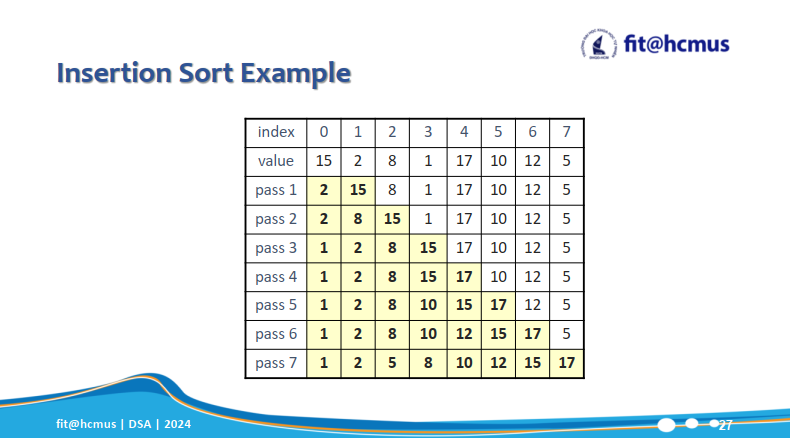
\includegraphics[scale=.40]{Figures/sort_demo/insertion.png}
    \caption{Insertion Sort Demo}
    \label{fig:enter-label}
\end{figure}
% \subsection{Shell Sort}

\subsubsection{Core concepts}
Shell sort is an enhanced version of insertion sort designed to address the problem of elements being far from their correct positions. Shell sort works by initially sorting elements that are far apart from each other, then progressively reducing the gap between elements to be compared. When gap is 1, it is an insertion-sort with nearly sorted array which makes the final pass much faster. This approach efficiently reduces the problem of elements being far from their correct positions, resulting in a quicker sorting process overall.

\vspace{10pt}

\subsubsection{Step-by-step Explanations}
\begin{itemize}[label=-]
    \item Step 1:Find the gap suitable for array, start by gap is equal to 1, gap multiplicate with 3 then plus 1, repeat this step if gap smaller than n. Then divide gap by 3 to find the largest gap that smaller than n.
    \item Step 2: Sort the elements in certain gap, use the idea of insertion-sort to sort the elements in certain gap ( start from i is equal to gap compare a[i] with a[i – gap]).
    \item Step 3: Divide gap by 3 then repeat step 2 until gap is equal to 1, it is an insertion-sort with the array is nearly sorted.
\end{itemize}

\subsubsection{Complexity Analysis}
\textbf{Time complexity analysis:} 
\begin{itemize}
    \item Best Case: $O(n \log n)$
    \item Average Case: Typically around $O(n^{5/4})$ to $O(n^{4/3})$
    \item Worst Case: $O(n^{3/2})$
\end{itemize}

\textbf{Space complexity analysis:} O(1) because it is an inplaced sorting algorithm

\vspace{10pt}

\subsubsection{Variants and Optimizations}
\textbf{Optimizations:} Depend on the data and the number of elements in array, we can choose suitable gap for having better performance. Two common ways to choose: 

\vspace{5pt}

Gap divide by 3: $..., 121, 40, 13, 4, 1$

\vspace{5pt}

Gap divide by 2: $..., 31, 15, 7, 3, 1$

\vspace{5pt}


\textbf{An example of Shell sort} ~\cite{ref1}

\begin{figure}[h]
    \centering
    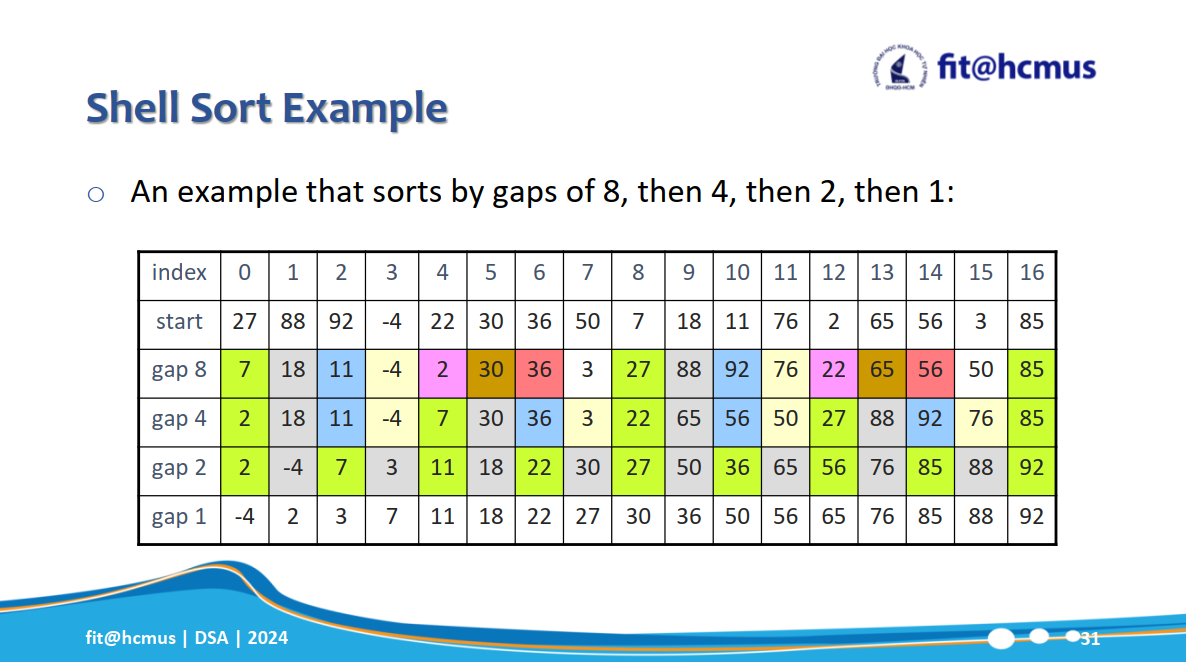
\includegraphics[scale=.23]{Figures/sort_demo/shell.png}
    \caption{Shell Sort Demo}
    \label{fig:enter-label}
\end{figure}
% \subsection{Bubble Sort}

\subsubsection{Core concept}
Bubble sort is also comparison-based sorting algorithm. The bubble sort compares adjacent items and exchanges them if they are out of order. This sort usually requires several passes over the data. ~\cite{ref7}

\vspace{5pt}

\subsubsection{Explanation}
\textbf{One way to explain this algorithm:}

Traverse from left and compare adjacent elements and the higher one is placed at right side. In this way, the largest element is moved to the rightmost end at first. This process is then continued to find the second largest and place it and so on until the data is sorted. ~\cite{ref9}

\vspace{5pt}

Lets consider the following array as an example: {29, 10, 14, 37, 13} ~\cite{ref7} 

\vspace{5pt}

\textbf{The first pass: }
Compare the items in the first pair 29 and 10 and exchange them because they are out of order. Next you consider the second pair 29 and 14 and exchange these items because they are out of order. The items in the third pair 29 and 37 are in order, and so you do not exchange them. Finally, you exchange the items in the last pair 37 and 13.

\vspace{5pt}

\textbf{The second pass:}
During the second pass of the bubble sort, return to the beginning of the array and consider pairs of items in exactly the same manner as the first pass. Do not, however, include the last and largest—item of the array. That is, the second pass considers the first n – 1 items of the array. After the second pass, the second-largest item in the array will be in its proper place in the next-to-last position of the array.

Now, ignoring the last two items, which are in order, continue with subsequent passes until the array is sorted.

The first two passes of a bubble sort of an array of five integers ~\cite{ref7}

\vspace{5pt}

\subsubsection{Complexity analysis}
\textbf{Time complexity:}
In each iteration of variable \(i\), the smallest element in the segment \(a[i \ldots n-1]\) will "bubble up" and be placed at \(a[i]\). Therefore, there are a total of \((n-1)\) iterations for variable \(i\).

Iteration 1: there are \((n-1)\) comparisons between \(a[j]\) and \(a[j-1]\), with \(j\) going from \(n-1\) to 1.

Iteration 2: there are \((n-2)\) comparisons between \(a[j]\) and \(a[j-1]\), with \(j\) going from \(n-2\) to 1.

...

Iteration \(n-1\): there is 1 comparison between \(a[1]\) and \(a[0]\).

Let \(f(n)\) be the number of comparisons and also the number of basic operations of the Bubble Sort algorithm, we have:

\[ f(n) = (n-1) + (n-2) + \ldots + 2 + 1 = \frac{n(n-1)}{2} \]

regardless of the distribution of the array elements.
\begin{itemize}
    \item Best case: $O(n)$ - Occurs when the original data is already sorted, it uses one pass, during which n – 1 comparisons and no exchanges occur. ~\cite{ref7}
    \item Average case: $O(n^2)$ - The algorithm always performs n-1 passes and involves n(n-1)/2 comparisons on average.
    \item Worst case: $O(n^2)$ - This occurs when the list is sorted in reverse order, requiring the maximum number of swaps.
\end{itemize}

\textbf{Space complexity:} $O(1)$ – Bubble sort is an in-place sorting algorithm, meaning it requires only a constant amount of additional memory space.

\vspace{5pt}

\subsubsection{Variants and optimizations}
\begin{itemize}[label=-]
    \item One common optimization is to introduce a flag that checks whether any swaps were made during a pass. If no swaps were made, the list is already sorted, and the algorithm can terminate early, improving the best-case time complexity to $O(n)$.
    \item Shaker sort is an extension of bubble sort, we will also discuss it later. It sorts in both directions in each pass through the list. By doing so, it can more quickly bring small values to the beginning and large values to the end, which helps reduce the number of passes needed compared to standard bubble sort.
\end{itemize}

\begin{figure}[h]
    \centering
    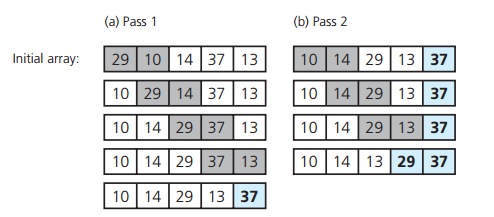
\includegraphics[scale=.80]{Figures/sort_demo/bubble.png}
    \caption{Bubble Sort Demo}
    \label{fig:enter-label}
\end{figure}

\vspace{10pt}
% \subsection{Heap Sort}

\subsubsection{Core concept}
Heap sort, as we have mentioned before, is an improvement of selection sort. It is comparison-based sorting technique based on heap data structure. We use heap to find the minimum element and place the minimum element at the beginning. Repeat the same process for the remaining elements.

\subsubsection{Explanation}
Heap definition (array-based representation) ~\cite{ref1}

\vspace{5pt}

Heap is a collection of $n$ elements ($a_0, a_1, \ldots, a_{n-1}$) in which every element (at position $i$) in the first half is greater than or equal to the elements at position $2i+1$ and $2i+2$.

\[
\text{for every } i \ (0 \leq i \leq n/2 - 1)
\]

\[
a_i \geq a_{2i + 1}
\]

\[
a_i \geq a_{2i + 2}
\]

Heap in above definition is called max-heap. (We also have min-heap structure)

\vspace{5pt}

Heap will reduce the time to find the minimum or maximum element when sorting the array which is an improvement of selection sort.

\textbf{Main steps:}
\begin{itemize}
    \item \textbf{Build a (max or min) Heap}: Convert the input array into a heap.
    \item \textbf{Heapify}: Rearrange the heap to maintain the max-heap property.
    \item \textbf{Extract Max Element}: Swap the first element (maximum) with the last element and reduce the heap size by one. Heapify the root to maintain the max-heap property.
    \item \textbf{Repeat}: Repeat the extraction process until the heap is empty.
\end{itemize}

The most important step is build a heap. Here is pseudo code for one way to build a max-heap. ~\cite{ref1}


\begin{algorithm}
\caption{Heap Construct}
\begin{verbatim}
1. Initialize index = floor(n/2) - 1
2. While index >= 0
     a. Call heapRebuild(index, a, n)
     b. index = index - 1
\end{verbatim}
\end{algorithm}

\begin{algorithm}
\caption{Heap Rebuild}
\begin{verbatim}
1. Initialize k = pos, v = a[k], isHeap = false
2. While not isHeap and 2k + 1 < n
     a. j = 2k + 1
     b. If j < n - 1
          i. If a[j] < a[j + 1]
               A. j = j + 1
     c. If a[k] >= a[j]
          i. isHeap = true
       else
          i. Swap a[k] and a[j]
          ii. k = j
\end{verbatim}
\end{algorithm}

\subsubsection{Complexity analysis}

\textbf{Time complexity:}
\begin{itemize}[label=-]
    \item Build max heap takes O(n) time and each of the n extraction takes O(log2 n)
    \item $O(n log_2 n)$ for all case
\end{itemize}

\textbf{Space complexity:} $O(1)$, if we don’t consider the recursive stack space. If we consider the recursive stack space then, in the worst case Heap sort could make $O(n)$.

\subsubsection{Variants and optimizations} 
Optimizing the heapify process can improve performance. For example, bottom-up heap construction can be more efficient than top-down heap construction.

\vspace{10pt}
% \subsection{Merge Sort}

\subsubsection{Core concept}
Merge sort uses the powerful strategy of divide and conquer. The array is repeatedly split into smaller subarrays then merging them together. During the merging process, the elements are compared and sorted to create larger sorted subarrays repeat this process until all subarrays are merged back into the original array, resulting in a fully sorted array. By breaking the problem into smaller and then combining the sorted pieces, merge sort efficiently sorts the entire array.

\vspace{3pt}

\subsubsection{Step-by-step Explanations}
\begin{itemize}[label=-]
    \item Step 1: Divide the Array into Subarrays by calling Recursive to split the array into smaller subarrays until each subarray has only 1 or 2 elements. This is achieved by continuously dividing the array into two halves.
    \item Step 2: Start merging the subarrays back together. Create two temporary arrays to hold the elements of the subarrays being merged. Compare the elements from the two temporary arrays and place the smaller element back into the original array. Continue merging and comparing until all elements are sorted and merged back into the original array.
\end{itemize}

\subsubsection{Complexity Analysis}
\textbf{Time complexity analysis: }
\begin{itemize}
    \item Best-case: $O(nlog(n))$
    \item Average-case: $O(nlog(n))$
    \item Worst-case: $O(nlog(n))$
\end{itemize}

\textbf{Space complexity analysis:} $O(n)$ because we have to create the many arrays with sum of these elements is equal to n elements of original array to merge.

\vspace{5pt}

\textbf{An example of merge sort:} ~\cite{ref2}

\begin{figure}[h]
    \centering
    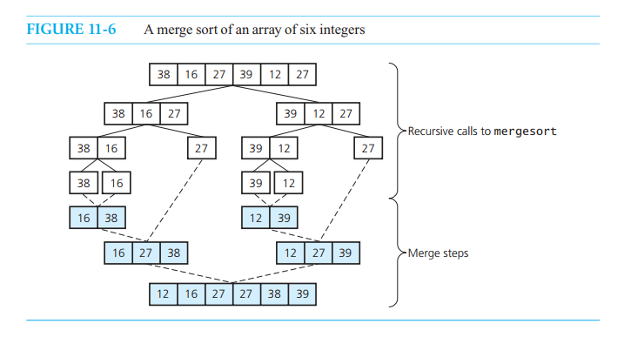
\includegraphics[scale=0.7]{Figures/sort_demo/merge.png}
    \caption{Merge Sort Demo}
    \label{fig:enter-label}
\end{figure}


% \subsection{Quick Sort}

\subsubsection{Core concept}
Quick sort is a sorting algorithm based on the Divide and Conquer algorithm that picks an element as a pivot and partitions the given array around the picked pivot by placing the pivot in its correct position in the sorted array. It one of best sorting algorithms using key comparisons. 

\subsubsection{Explanation}

The algorithm consists of the following three steps: ~\cite{ref1}
\begin{itemize}[label=-]
    \item Divide: Partition the list.
    \begin{itemize}[label=$\bullet$]
        \item To partition the list, we first choose some element from the list for which we hope about half the elements will come before and half after. Call this element the pivot.
        \item Then we partition the elements so that all those with values less than the pivot come in one sub-list and all those with greater values come in another.
    \end{itemize}
    \item Recursion: Recursively sort the sub-lists separately.
    \item Conquer: Put the sorted sub-lists together.
\end{itemize}


\textbf{One partition technique} ~\cite{ref1}
\begin{figure}[h]
\centering
\begin{minipage}{0.45\textwidth}
    \centering
    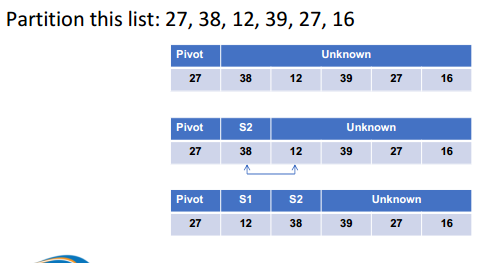
\includegraphics[scale=0.6]{Figures/sort_demo/quick_1.png}
    \caption{Partition technique}
    \label{fig:before_undo}
\end{minipage}\hfill
\begin{minipage}{0.45\textwidth}
    \centering
    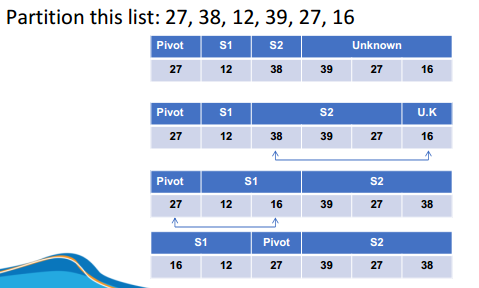
\includegraphics[scale=0.6]{Figures/sort_demo/quick_2.png}
    \caption{Partition technique}
    \label{fig:after_undo}
\end{minipage}
\end{figure}


\vspace{10pt}

\textbf{Another partition technique} ~\cite{ref7} 
\begin{figure}[h]
    \centering
    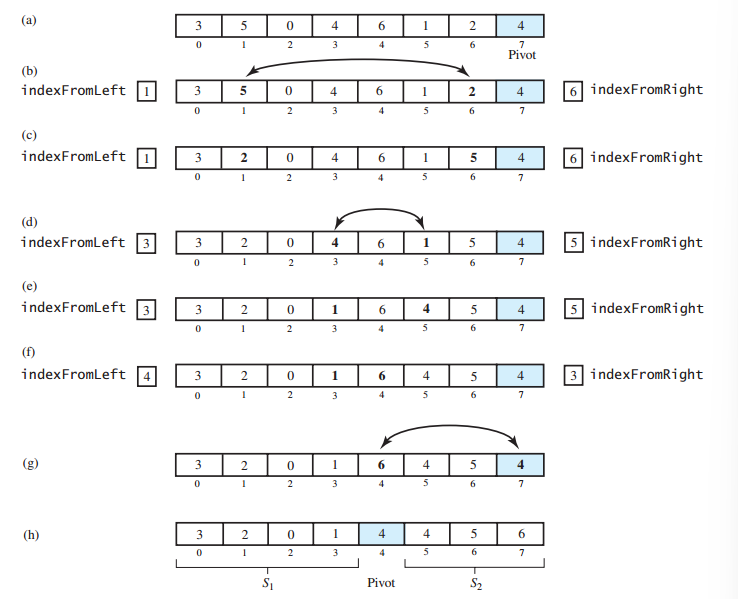
\includegraphics[width=0.55\textwidth]{Figures/sort_demo/quick_3.png}
    \caption{Partition technique 2}
    \label{fig:enter-label}
\end{figure}

\newpage

As the partition process is done recursively, it keeps on putting the pivot in its actual position in the sorted array. Repeatedly putting pivots in their actual position makes the array sorted.

\subsubsection{Complexity analysis}

\textbf{Time complexity:}
\begin{itemize}
    \item Best case: O(n log2n)  - occur when the pivot chosen at the each step divides the array into roughly equal halves, make balanced partitions, leading to efficient sorting.
    \item Average case: O(n log2n)
    \item Worst case: $O(n^2)$ - This rarely occurs when the pivot selection is poor, leading to unbalanced partitions (e.g., when the array is already sorted, and the first or last element is chosen as the pivot).
\end{itemize}

\textbf{Space complexity:} $O(1)$, if we don’t consider the recursive stack space. If we consider the recursive stack space then, in the worst case quicksort could make $O(n)$. ~\cite{ref10}

\subsubsection{Variants and optimizations}
\begin{itemize}[label=-]
    \item Median of three pivot selection: This pivot selection scheme assumes that the array has at least three entries. If you have only three entries, the pivot selection sorts them, so there is no need for the partition method or for a quick. ~\cite{ref7}
    \item Tail call optimization: partition function is in-place, but we need extra space for recursive function calls. Optimizing the recursive calls to minimize the depth of the recursive stack. By always sorting the smaller subarray first and using tail recursion for the larger subarray, the stack depth can be reduced.
\end{itemize}

\vspace{10pt}
% \subsection{Radix Sort}

\subsubsection{Core Concepts}
Radix sort is an algorithm that does not use comparisons to sorted the array. To be specific, treats each data item as a character string, groups the data items according to the rightmost character then put these groups into order with respect to this rightmost character, combine all the groups and move to the next left position. At the end, the sort operation will be in sorted. ~\cite{ref1}

\vspace{3pt}

\subsubsection{Step-by-step Explaination}
\begin{itemize}[label=-]
    \item Step 1: find max value by calling getMax to determine the maximum number in the array.
    \item Step 2: Start with the rightmost significant number. Apply countSort to sort the array based on the current number. Move to the next significant digit by multiplying exp by 10. Repeat the process until all digits have been processed (when m / exp becomes 0).
\end{itemize}

\subsubsection{Complexity Analysis}
\textbf{Time Complexity: }
\begin{itemize}
    \item Radix sort is a non-comparative integer sorting algorithm that sorts data with integer keys by grouping the keys by the individual digits which share the same significant position and value. It has a time complexity of $O(d \cdot (n + b))$, where d is the number of digits, n is the number of elements, and b is the base of the number system being used.
    \item In practical implementations, radix sort is often faster than other comparison-based sorting algorithms, such as quicksort or merge sort, for large datasets, especially when the keys have many digits. However, its time complexity grows linearly with the number of digits, and so it is not as efficient for small datasets. ~\cite{ref5}
\end{itemize}

\textbf{Space complexity: }
Radix sort also has a space complexity of $O(n + b)$, where n is the number of elements and b is the base of the number system. This space complexity comes from the need to create buckets for each digit value and to copy the elements back to the original array after each digit has been sorted.

\textbf{An example of radix sort:} ~\cite{ref2}

\begin{figure}[h]
    \centering
    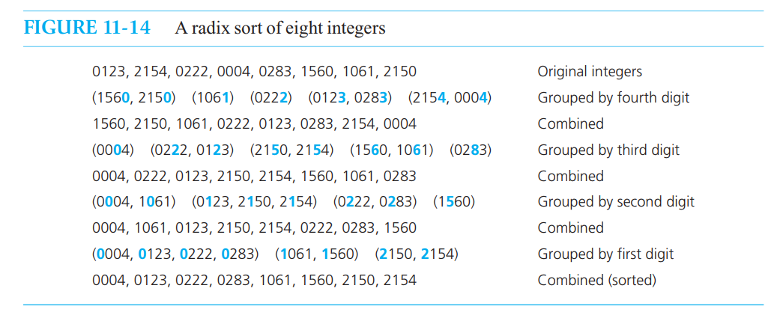
\includegraphics[width=1.\textwidth]{Figures/sort_demo/radix.png}
    \caption{Radix Sort Demo}
    \label{fig:enter-label}
\end{figure}
% \subsection{Counting Sort}

\subsubsection{Core Concepts}
Counting sort is an efficient algorithm for sorting integers. It works by counting the number of occurrences of each distinct value in the input array using a separate count array. These counts are then used to place the elements back into the original array in sorted order, ranging from the smallest to the largest value. This method ensures that the array is sorted correctly and efficiently. ~\cite{ref3}
\subsubsection{Step-by-step Explanations}
\begin{itemize}[label=-]
    \item Step 1: find max value of the array
    \item Step 2: create an array with max value of elements to count appearances
    \item Step 3: iterate through the original array a. For each element in a, increment the corresponding index in the count array b. This effectively counts the occurrences of each element.
    \item Step 4: assign the value back to original array
\end{itemize}

\subsubsection{Complexity Analysis}
\textbf{Time Complexity:}
\begin{itemize}
    \item Best-case: $O(n + k)$
    \item Average-case: $O(n + k)$
    \item Worst-case: $O(n + k)$
    \item where n is the number of elements in the array, and k is the range of the input.
\end{itemize}

\textbf{Space Complexity:} $O(n + k)$ because it requires additional space for the count array and the output array.

\subsubsection{Variants and Optimizations}
\textbf{Negative number:} if there are negative numbers in input array and there is no negative index so we can plus to all elements of the array by the smallest value to make sure that smallest is 0 then running counting and the final sorted array, we minus all elements by the value that we plus in first step.

\vspace{10pt}

% \subsection{Binary Insertion Sort}

\subsubsection{Core concept}
Binary Insertion sort is a variation of insertion sort. the core idea is similar to insertion sort, but instead of using linear search to find the position where an element should be inserted, this algorithm uses binary search. Thus, it reduce the comparative value of inserting a single element. ~\cite{ref8}

\subsubsection{Explanation}
The algorithm is similar to insertion sort algorithm, but here we use binary search to find the position:
\begin{itemize}[label=-]
    \item \textbf{Initialization:} Start with the second element (index 1) of the array, as the first element is considered sorted.
    \item \textbf{Binary Search for Position:} Use binary search to determine the correct position in the sorted portion of the array for the current element.
    \item \textbf{Shift Elements:} Shift elements to the right to make room for the current element.
    \item \textbf{Insert Element:} Insert the current element into its correct position.
    \item \textbf{Repeat:} Repeat the process for each element in the array until the entire array is sorted
\end{itemize}

\textbf{Step-by-step:}
\begin{itemize}[label=-]
    \item Lets use the array as an example {29, 10, 14, 37, 13}

    \item Consider 29 is in sorted part, start from 10, we use binary search to find the position in sorted part to insert 10. 10 smaller than 29 so the position is 0. Then we shift and insert 10.

    \item After first insertion {10, 29, 14, 37, 13}

    \item Continue to find the location for 14 which is between 10 and 29. We shift and insert 14 to the correct position.

    \item After second insertion {10, 14, 29, 37, 13}

    \item We continue to the same technique for 37 and 13. Finally, we get a sorted list

    \item After third and fourth insertions {10, 13, 14, 29, 37}
\end{itemize}


\subsubsection{Complexity analysis}

\textbf{Time complexity:}
Consider the array $a[]$ sorted in increasing order.

\textbf{Iteration 1:} requires 1 comparison

\textbf{Iteration 2:} requires $\log 2 + 1$ comparisons

...

\textbf{Iteration $n - 1$:} requires $\log(n - 1) + 1$ comparisons

In all iterations, since the array is already sorted in increasing order, the elements do not need to be moved.

\[
f(n) = 1 + \log 2 + 1 + \log 3 + 1 + \ldots + \log(n - 1) + 1 = n - 1 + \sum_{i=2}^{n-1} \log i
\]

Consider \(\displaystyle \sum_{i=2}^{n-1} \log i \approx \sum_{i=1}^{n} \log i \), then:

\[
\sum_{i=n/2}^{n} \log \frac{n}{2} \leq \sum_{i=1}^{n} \log i \leq \sum_{i=1}^{n} \log n \Rightarrow \frac{n}{2} \log \frac{n}{2} \leq f(n) \leq n \log n
\]

Thus, $f(n) \in \Omega(n \log n)$ and $f(n) \in O(n \log n)$, therefore $f(n) \in \Theta(n \log n)$.

Therefore, if we only apply simple binary search, in the best case, the complexity of BinaryInsertionSort is $O(n \log n)$. This can be improved by comparing $a[i]$ and $a[i-1]$ first when performing the binary search, which can reduce it to $O(n)$.
\begin{itemize}
    \item Best Case: $O(n log n)$ – Binary search reduces the number of comparisons, but shifting elements still takes linear time.
    \item Average Case: $O(n^2)$ – Despite using binary search, the time complexity remains quadratic due to the shifting of elements.
    \item Worst Case: $O(n^2$) – Similar to the average case, the need to shift elements results in quadratic time complexity.
\end{itemize}

\textbf{Space complexity:} \textbf{O(1)} - binary insertion sort is similar to insertion sort.  It is an in-place sorting algorithm, meaning it requires only a constant amount of additional memory space.

\subsubsection{Variants and optimizations}
Tim Sort is a hybrid sorting algorithm derived from merge sort and insertion sort. It was designed to perform well on many kinds of real-world data. ~\cite{ref11}

\vspace{10pt}
% \subsection{Shaker Sort}

\subsubsection{Core concept}
Shaker sort, also known as cocktail sort or bidirectional bubble sort, is a variation of bubble sort that sorts the array in both directions on each pass through the list. This means it traverses the array from left to right and then from right to left, ensuring that the largest elements "bubble" to the end and the smallest elements "bubble" to the beginning of the array.

\subsubsection{Explanation}

The algorithm is broken up into 2 stages: ~\cite{ref12}
\begin{itemize}[label=-]
    \item The first stage loops through the array from left to right, just like the Bubble Sort. During the loop, adjacent items are compared and if the value on the left is greater than the value on the right, then values are swapped. At the end of the first iteration, the largest number will reside at the end of the array.
    \item The second stage loops through the array in opposite direction- starting from the item just before the most recently sorted item, and moving back to the start of the array. Here also, adjacent items are compared and are swapped if required.
\end{itemize}

\vspace{5pt}

\textbf{Example for the first pass} ~\cite{ref12}

Let us consider an example array: (5 1 4 2 8 0 2)

\textbf{First Forward Pass:}

\begin{lstlisting}[mathescape=true]
(5 1 4 2 8 0 2) $\rightarrow$ (1 5 4 2 8 0 2), Swap since 5 > 1
(1 5 4 2 8 0 2) $\rightarrow$ (1 4 5 2 8 0 2), Swap since 5 > 4
(1 4 5 2 8 0 2) $\rightarrow$ (1 4 2 5 8 0 2), Swap since 5 > 2
(1 4 2 5 8 0 2) $\rightarrow$ (1 4 2 5 8 0 2)
(1 4 2 5 8 0 2) $\rightarrow$ (1 4 2 5 0 8 2), Swap since 8 > 0
(1 4 2 5 0 8 2) $\rightarrow$ (1 4 2 5 0 2 8), Swap since 8 > 2
\end{lstlisting}

After the first forward pass, the greatest element of the array will be present at the last index of the array.

\vspace{10pt}

\textbf{First Backward Pass:}

\begin{lstlisting}[mathescape=true]
(1 4 2 5 0 2 8) $\rightarrow$ (1 4 2 5 0 2 8)
(1 4 2 5 0 2 8) $\rightarrow$ (1 4 2 0 5 2 8), Swap since 5 > 0
(1 4 2 0 5 2 8) $\rightarrow$ (1 4 0 2 5 2 8), Swap since 2 > 0
(1 4 0 2 5 2 8) $\rightarrow$ (1 0 4 2 5 2 8), Swap since 4 > 0
(1 0 4 2 5 2 8) $\rightarrow$ (0 1 4 2 5 2 8), Swap since 1 > 0
\end{lstlisting}

After the first backward pass, the smallest element of the array will be present at the first index of the array.

\subsubsection{Complexity analysis}

\textbf{Time complexity:}
\begin{itemize}
    \item Best Case: $O(n)$ – This occurs when the array is already sorted. Only one full pass through the array is needed.
    \item Average Case: $O(n^2)$ – Each element needs to be compared with many other elements in the array.
    \item Worst Case: $O(n^2)$ – Similar to the average case, the worst-case scenario involves multiple passes through the array with numerous swaps.
\end{itemize}

\textbf{Space complexity:} $O(1)$ – Shaker sort is an in-place sorting algorithm, meaning it requires only a constant amount of additional memory space.

\vspace{10pt}
% \subsection{Flash Sort}

\subsubsection{Core Concepts}
Flash sort is sorting that divide elements in to different buckets which the gap of value is smallest and make sure that the largest value in previous bucket is smaller that lowest value in next bucket. Then we use basic sorting algorithms to sort buckets, often use insertion sort because it work well with nearly sorted array. ~\cite{ref4}

\subsubsection{Step-by-step Explanations}
First, calculate the number of buckets by multiplying the size of the input array by 0.45. Then, create an array to count the number of elements in each bucket. Iterate through the input array, assigning each element to the appropriate bucket. Next, adjust the bucket counts to reflect the final positions of elements. Reorder the elements so each bucket contains the correct values. Finally, apply insertion sort within each bucket to sort the elements, resulting in a fully sorted array.

\subsubsection{Complexity Analysis}
\textbf{Time Complexity:}
\begin{itemize}
    \item Best-case: $O(n)$
    \item Average-case: $O(n + k)$
    \item Worst-case: $O(n + k)$
    \item Where n is the number of elements, and k is the number of buckets.
\end{itemize}

\textbf{Space Complexity:} $O(n + k)$ because it requires additional space for the count array and the class boundaries.

\subsubsection{Variants and Optimizations}
There are different way to count the number of buckets based on the different data so just test and find suitable buckets to improve performance, sometimes number of buckets equal to $0.45 * n or 0.42 * n or k * n$. We can use quick-sort instead of insertion-sort if the array is larger. 


% \newpage

% \section{Survey and Evaluation}
% \subsection{Randomize Data}
\subsubsection{Time}
Execution time unit: milliseconds

\begin{table}[h!]
\centering
\begin{tabular}{|l|r|r|r|r|r|r|}
\hline
\textbf{Algorithm} & \textbf{10,000} & \textbf{30,000} & \textbf{50,000} & \textbf{100,000} & \textbf{300,000} & \textbf{500,000} \\ \hline
selection-sort & 90.9034 & 819.165 & 2144.86 & 8596.38 & 76158.2 & 210088 \\ \hline
insertion-sort & 5.4657 & 49.4609 & 138.977 & 547.006 & 4937.82 & 13827.8 \\ \hline
shell-sort & 20.9348 & 204.922 & 550.198 & 2260.1 & 18522.9 & 53320.1 \\ \hline
bubble-sort & 97.1671 & 1116.17 & 3208.09 & 13295.4 & 121053 & 339611 \\ \hline
heap-sort & 0.909 & 3.1648 & 5.3967 & 11.5898 & 39.6501 & 68.36 \\ \hline
merge-sort & 3.2503 & 9.3788 & 15.4051 & 28.9049 & 87.508 & 146.323 \\ \hline
quick-sort & 0.5708 & 1.7461 & 3.1067 & 6.3324 & 20.1092 & 34.9733 \\ \hline
radix-sort & 1.8813 & 0.5193 & 0.7778 & 1.8149 & 4.8387 & 8.4334 \\ \hline
counting-sort & 0.07 & 0.1945 & 0.2539 & 0.4312 & 0.902 & 1.3383 \\ \hline
binary-insertion-sort & 4.8785 & 37.591 & 102.974 & 410.325 & 3620.11 & 10357.5 \\ \hline
shaker-sort & 85.7846 & 842.283 & 2380.6 & 9535.75 & 86159.8 & 239150 \\ \hline
flash-sort & 0.1696 & 0.6379 & 0.9506 & 1.8552 & 7.8633 & 16.1854 \\ \hline
\end{tabular}
\label{table:running_time}
\end{table}

\begin{figure}[h]
    \centering
    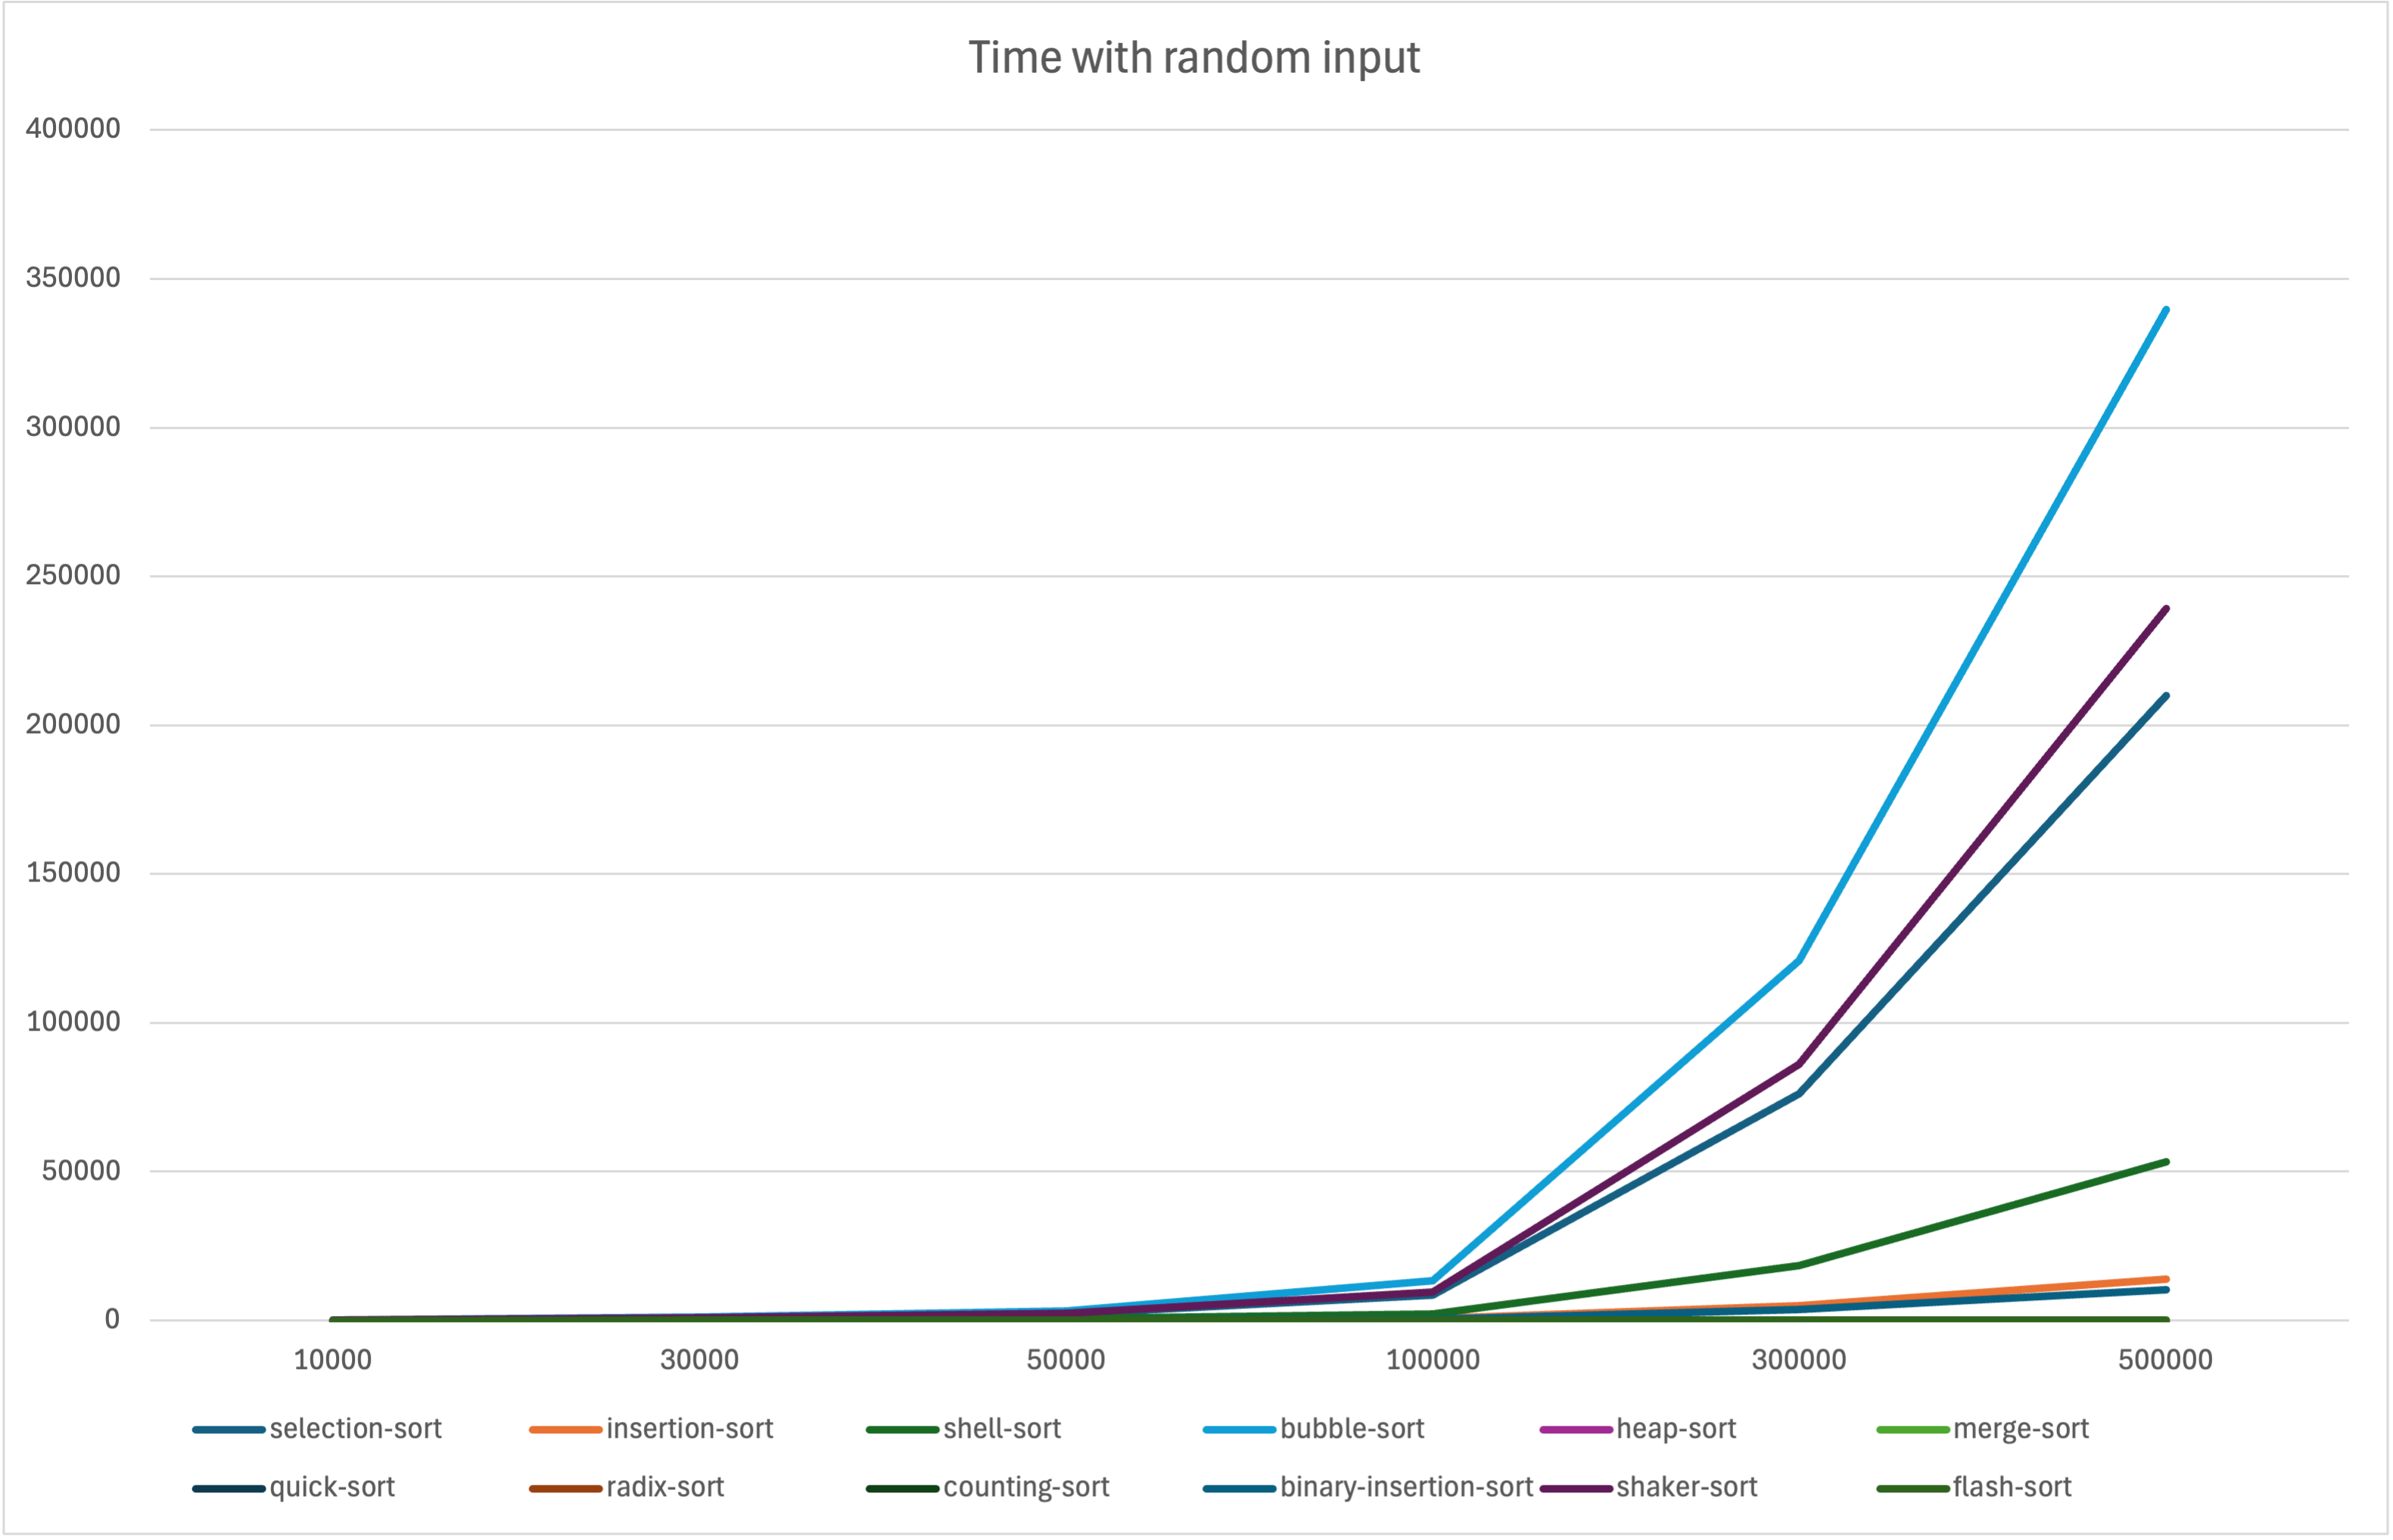
\includegraphics[scale=0.65]{Figures/Visualization/Random_time.png}
    \caption{Execution time for Randomize data}
    \label{fig:enter-label}
\end{figure}

\textbf{Comments on the running time of sorting algorithms with random data}
\begin{enumerate}
    \item \textbf{Fastest algorithms:} \\
   - \texttt{Counting Sort}, \textit{Quick Sort}, \textit{Heap Sort}, and \textit{Flash Sort} are the fastest algorithms as the data size increases. Notably, \textit{Quick Sort} and \textit{Flash Sort} have very low running times compared to other algorithms, even with large datasets like 500,000 elements.

    \item \textbf{Slowest algorithms:} \\
   - \textit{Bubble Sort}, \textit{Selection Sort}, and \textit{Insertion Sort} have the longest running times. \textit{Bubble Sort} and \textit{Selection Sort} have rapidly increasing running times, reaching hundreds of thousands of seconds with datasets of 500,000 elements.

    \item \textbf{Other algorithms:} \\
   - \textit{Merge Sort}, \textit{Shell Sort}, and \textit{Shaker Sort} have average running times, neither too fast nor too slow.
\end{enumerate}

\subsubsection{Comparison}
\begin{table}[h!]
\centering
\begin{tabular}{|l|r|r|r|r|r|r|}
\hline
\textbf{Algorithm} & \textbf{10,000} & \textbf{30,000} & \textbf{50,000} & \textbf{100,000} & \textbf{300,000} & \textbf{500,000} \\ \hline
selection-sort & 100020001 & 900060001 & 2500100001 & 10000200001 & 90000600001 & 250000000001 \\ \hline
insertion-sort & 49650481 & 448332712 & 1248140892 & 4990403035 & 45011022554 & 124964111984 \\ \hline
shell-sort & 136486703 & 1228074234 & 3411144570 & 13643867417 & 1.2279e+11 & 3.41082e+11 \\ \hline
bubble-sort & 100009999 & 900029999 & 2500049999 & 10000099999 & 90000299999 & 2.5e+11 \\ \hline
heap-sort & 638069 & 2149637 & 3772566 & 8044375 & 26494137 & 45968203 \\ \hline
merge-sort & 583723 & 1937626 & 3383060 & 7166134 & 23383144 & 40382087 \\ \hline
quick-sort & 364891 & 1086464 & 1921044 & 4144209 & 14922110 & 27756867 \\ \hline
radix-sort & 140051 & 510064 & 850064 & 1700064 & 510064 & 850064 \\ \hline
counting-sort & 60001 & 180001 & 265539 & 465539 & 1265539 & 2065539 \\ \hline
binary-insertion-sort & 25432305 & 226953151 & 629328887 & 2511144485 & 22498338748 & 62537270911 \\ \hline
shaker-sort & 66785983 & 599351162 & 1667586501 & 6658782743 & 60022078477 & 1.66739e+11 \\ \hline
flash-sort & 92801 & 285860 & 496012 & 892630 & 2755320 & 4583014 \\ \hline
\end{tabular}
\label{table:comparisons}
\end{table}

\begin{figure}[h]
    \centering
    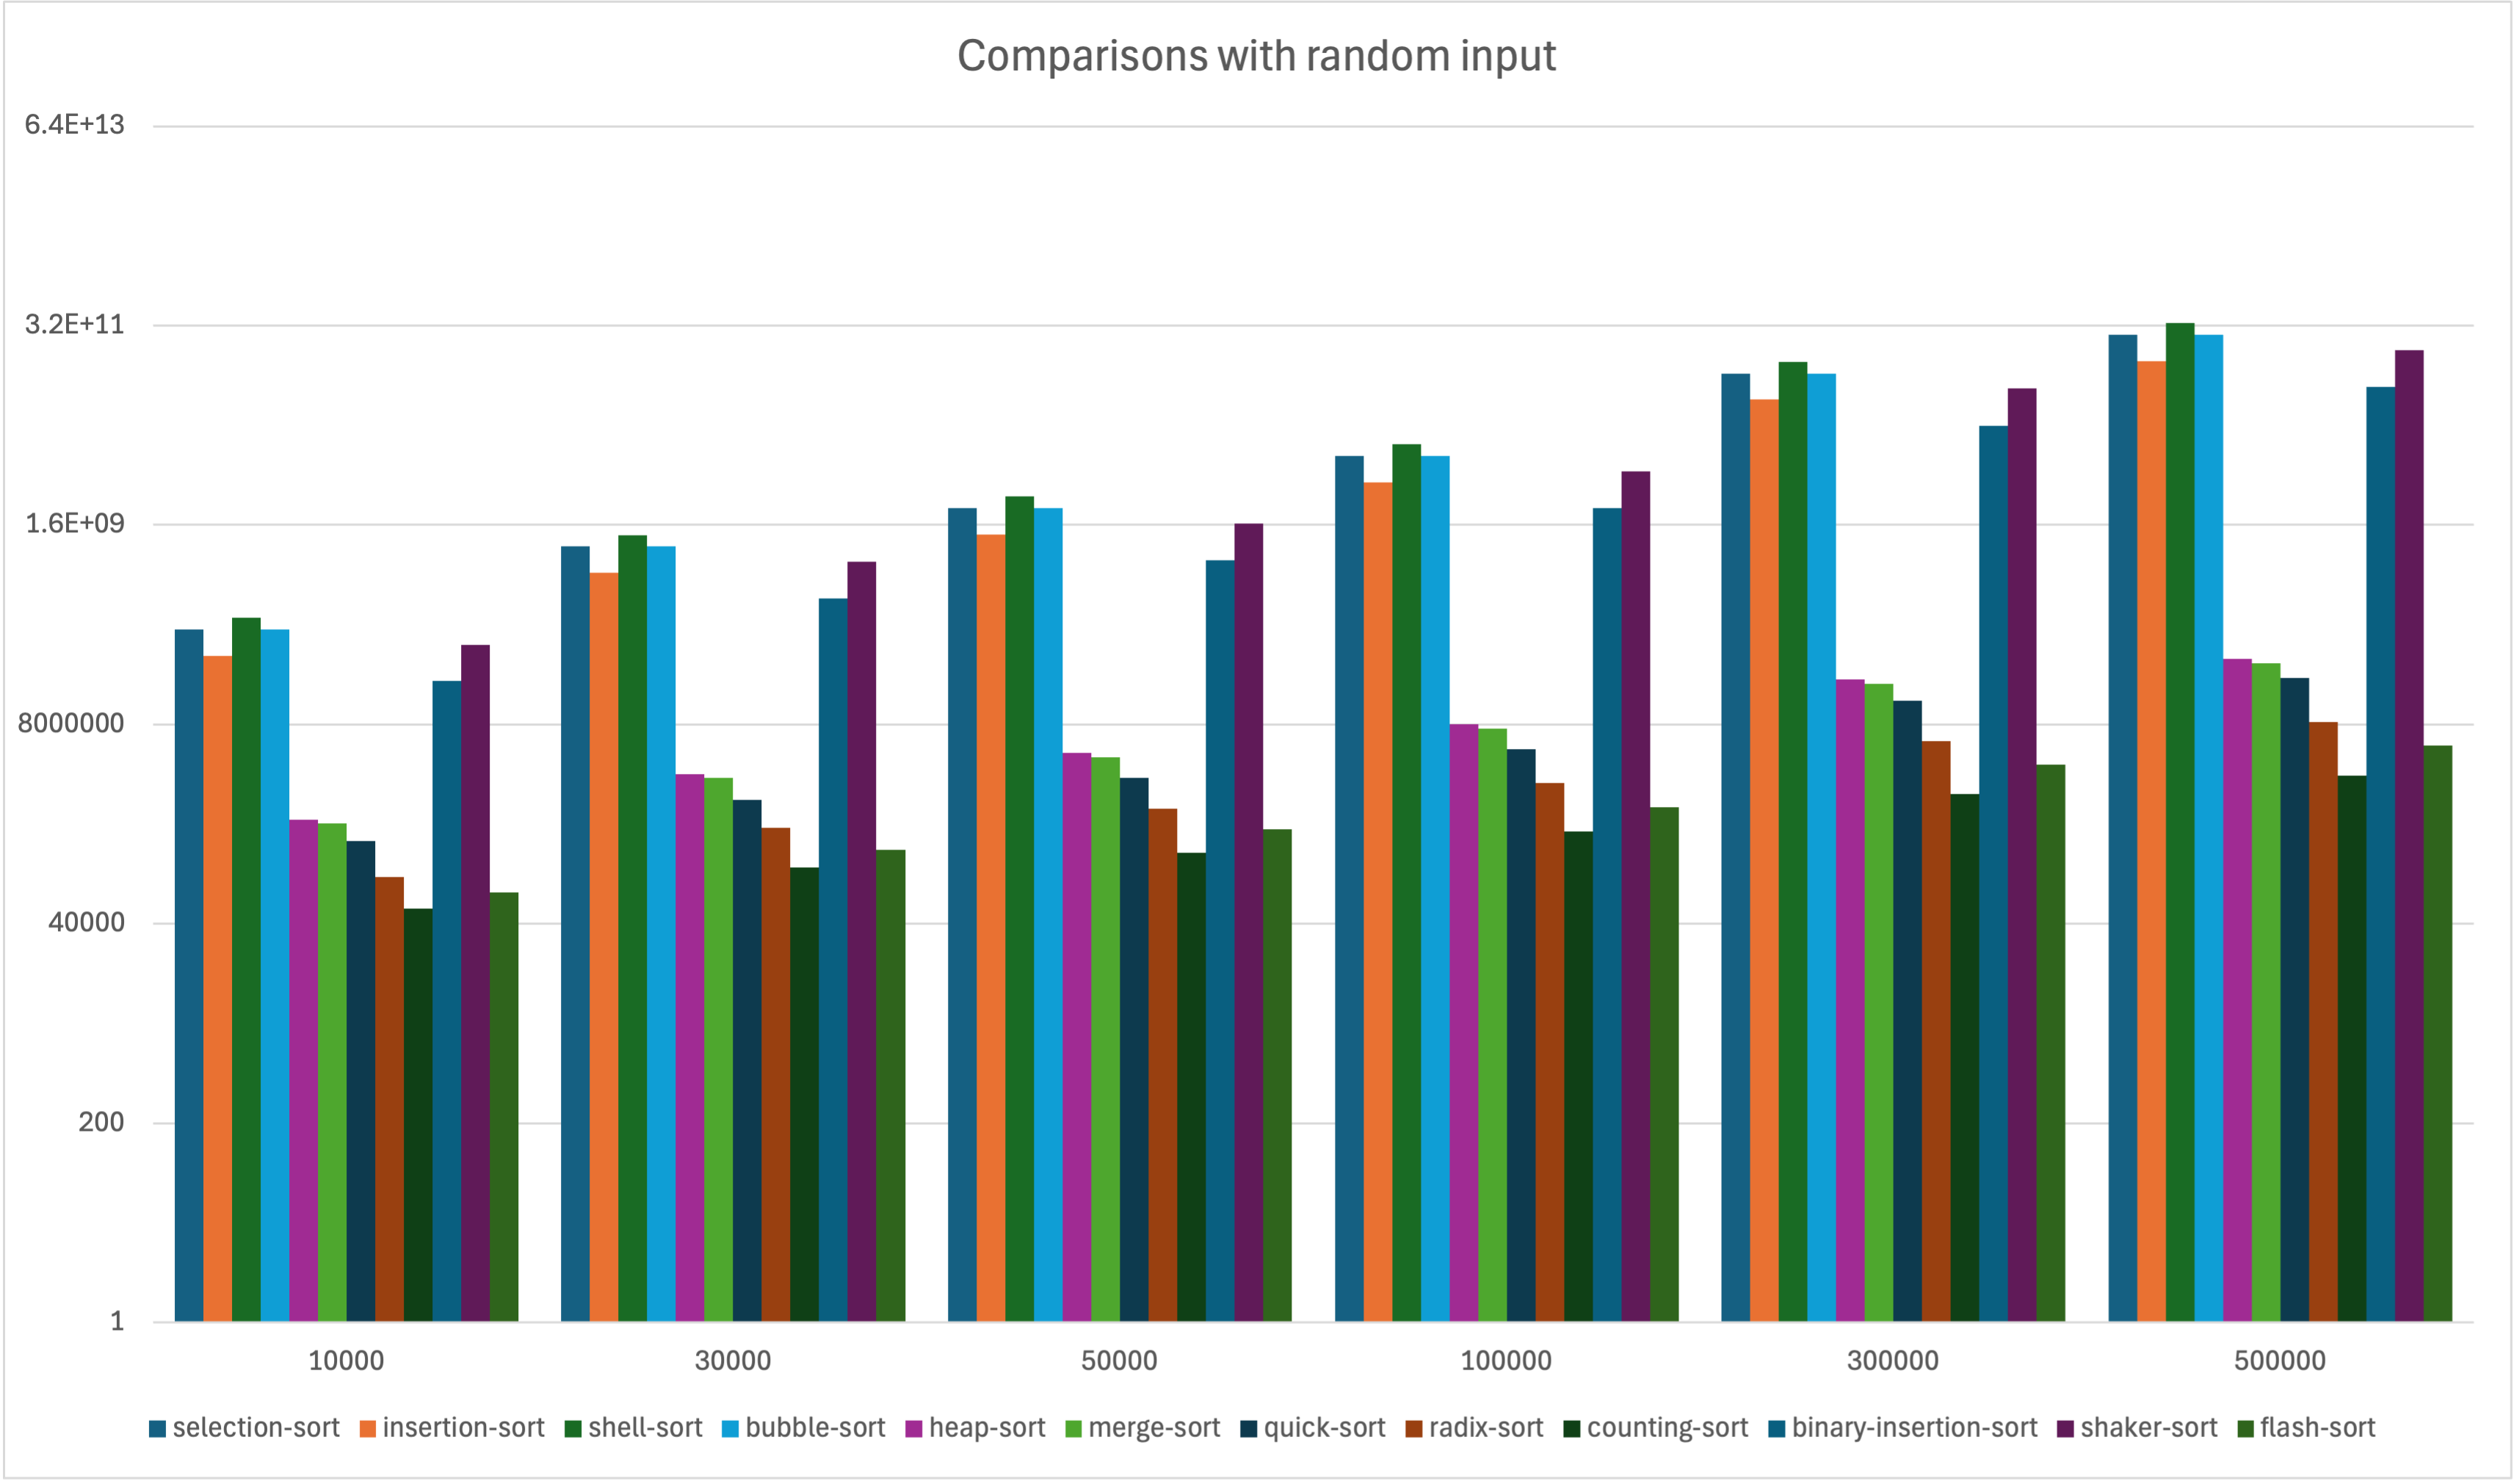
\includegraphics[scale=0.65]{Figures/Visualization/Random_compare.png}
    \caption{Number of comparisons of the algorithm for Randomize data}
    \label{fig:enter-label}
\end{figure}

\textbf{Comments on the number of comparisons of sorting algorithms with random data}
\begin{enumerate}
    \item \textbf{Fewest comparisons:} \\
   - \textit{Counting Sort}, \textit{Flash Sort}, and \textit{Radix Sort} have the fewest comparisons, especially \textit{Counting Sort}, which has very low comparison counts even with large datasets.

    \item \textbf{Most comparisons:} \\
   - \textit{Bubble Sort}, \textit{Selection Sort}, and \textit{Insertion Sort} have very high comparison counts, especially \textit{Bubble Sort} and \textit{Selection Sort}, which reach billions of comparisons with datasets of 500,000 elements.

    \item \textbf{Other algorithms:} \\
   - \textit{Quick Sort}, \textit{Heap Sort}, and \textit{Merge Sort} have relatively low comparison counts, making them more efficient compared to slower sorting algorithms.
\end{enumerate}

\subsubsection{Overall}
\textbf{Overall comments on algorithms based on all data and size}

\begin{enumerate}
    \item \textbf{Overall fastest algorithms:} \\
   - \textit{Quick Sort}, \textit{Heap Sort}, and \textit{Flash Sort} are the overall fastest algorithms. Among them, \textit{Quick Sort} is most commonly used due to its efficiency in handling large datasets.

    \item \textbf{Overall slowest algorithms:} \\
   - \textit{Bubble Sort}, \textit{Selection Sort}, and \textit{Insertion Sort} are the overall slowest algorithms. They are suitable only for very small datasets or educational purposes.

    \item \textbf{Stable and unstable algorithms:} \\
   - Algorithms like \textit{Merge Sort} and \textit{Insertion Sort} are stable, meaning they maintain the relative order of equal elements. \\
   - Algorithms like \textit{Quick Sort} and \textit{Heap Sort} are unstable, meaning they do not maintain the relative order of equal elements.
\end{enumerate}

% \subsection{Sorted Data}
\subsubsection{Time}
Execution time unit: milliseconds

\begin{table}[h!]
\centering
\begin{tabular}{|l|r|r|r|r|r|r|}
\hline
\textbf{Algorithm} & \textbf{10000} & \textbf{30000} & \textbf{50000} & \textbf{100000} & \textbf{300000} & \textbf{500000} \\
\hline
Selection Sort & 83.5349 & 762.314 & 2093.73 & 8438.43 & 75874.9 & 210401 \\ \hline
Insertion Sort & 0.0043 & 0.013 & 0.0228 & 0.0452 & 0.1466 & 0.2558 \\ \hline
Shell Sort & 15.9199 & 166.915 & 454.441 & 1746.54 & 16108.9 & 72609.4 \\ \hline
Bubble Sort & 13.4474 & 123.507 & 329.481 & 1383.44 & 12187 & 34030.9 \\ \hline
Heap Sort & 0.691 & 2.2718 & 3.8386 & 8.0435 & 26.315 & 44.2006 \\ \hline
Merge Sort & 2.336 & 7.0626 & 11.8658 & 23.7198 & 73.8943 & 119.809 \\ \hline
Quick Sort & 78.4909 & 699.612 & 1986.74 & 7702.21 & 69509.3 & 198334 \\ \hline
Radix Sort & 0.1545 & 0.4646 & 0.943 & 1.5853 & 6.1696 & 10.6871 \\ \hline
Counting Sort & 0.016 & 0.0444 & 0.0809 & 0.208 & 0.7713 & 1.0371 \\ \hline
Binary Insertion Sort & 0.242 & 0.8476 & 1.3542 & 2.9678 & 10.6128 & 17.5126 \\ \hline
Shaker Sort & 0.0036 & 0.0094 & 0.0166 & 0.0418 & 0.1131 & 0.2715 \\ \hline
Flash Sort & 0.0948 & 0.2717 & 0.6822 & 1.1887 & 3.7231 & 5.9786 \\
\hline
\end{tabular}
\label{table:execution_time}
\end{table}

\begin{figure}[h]
    \centering
    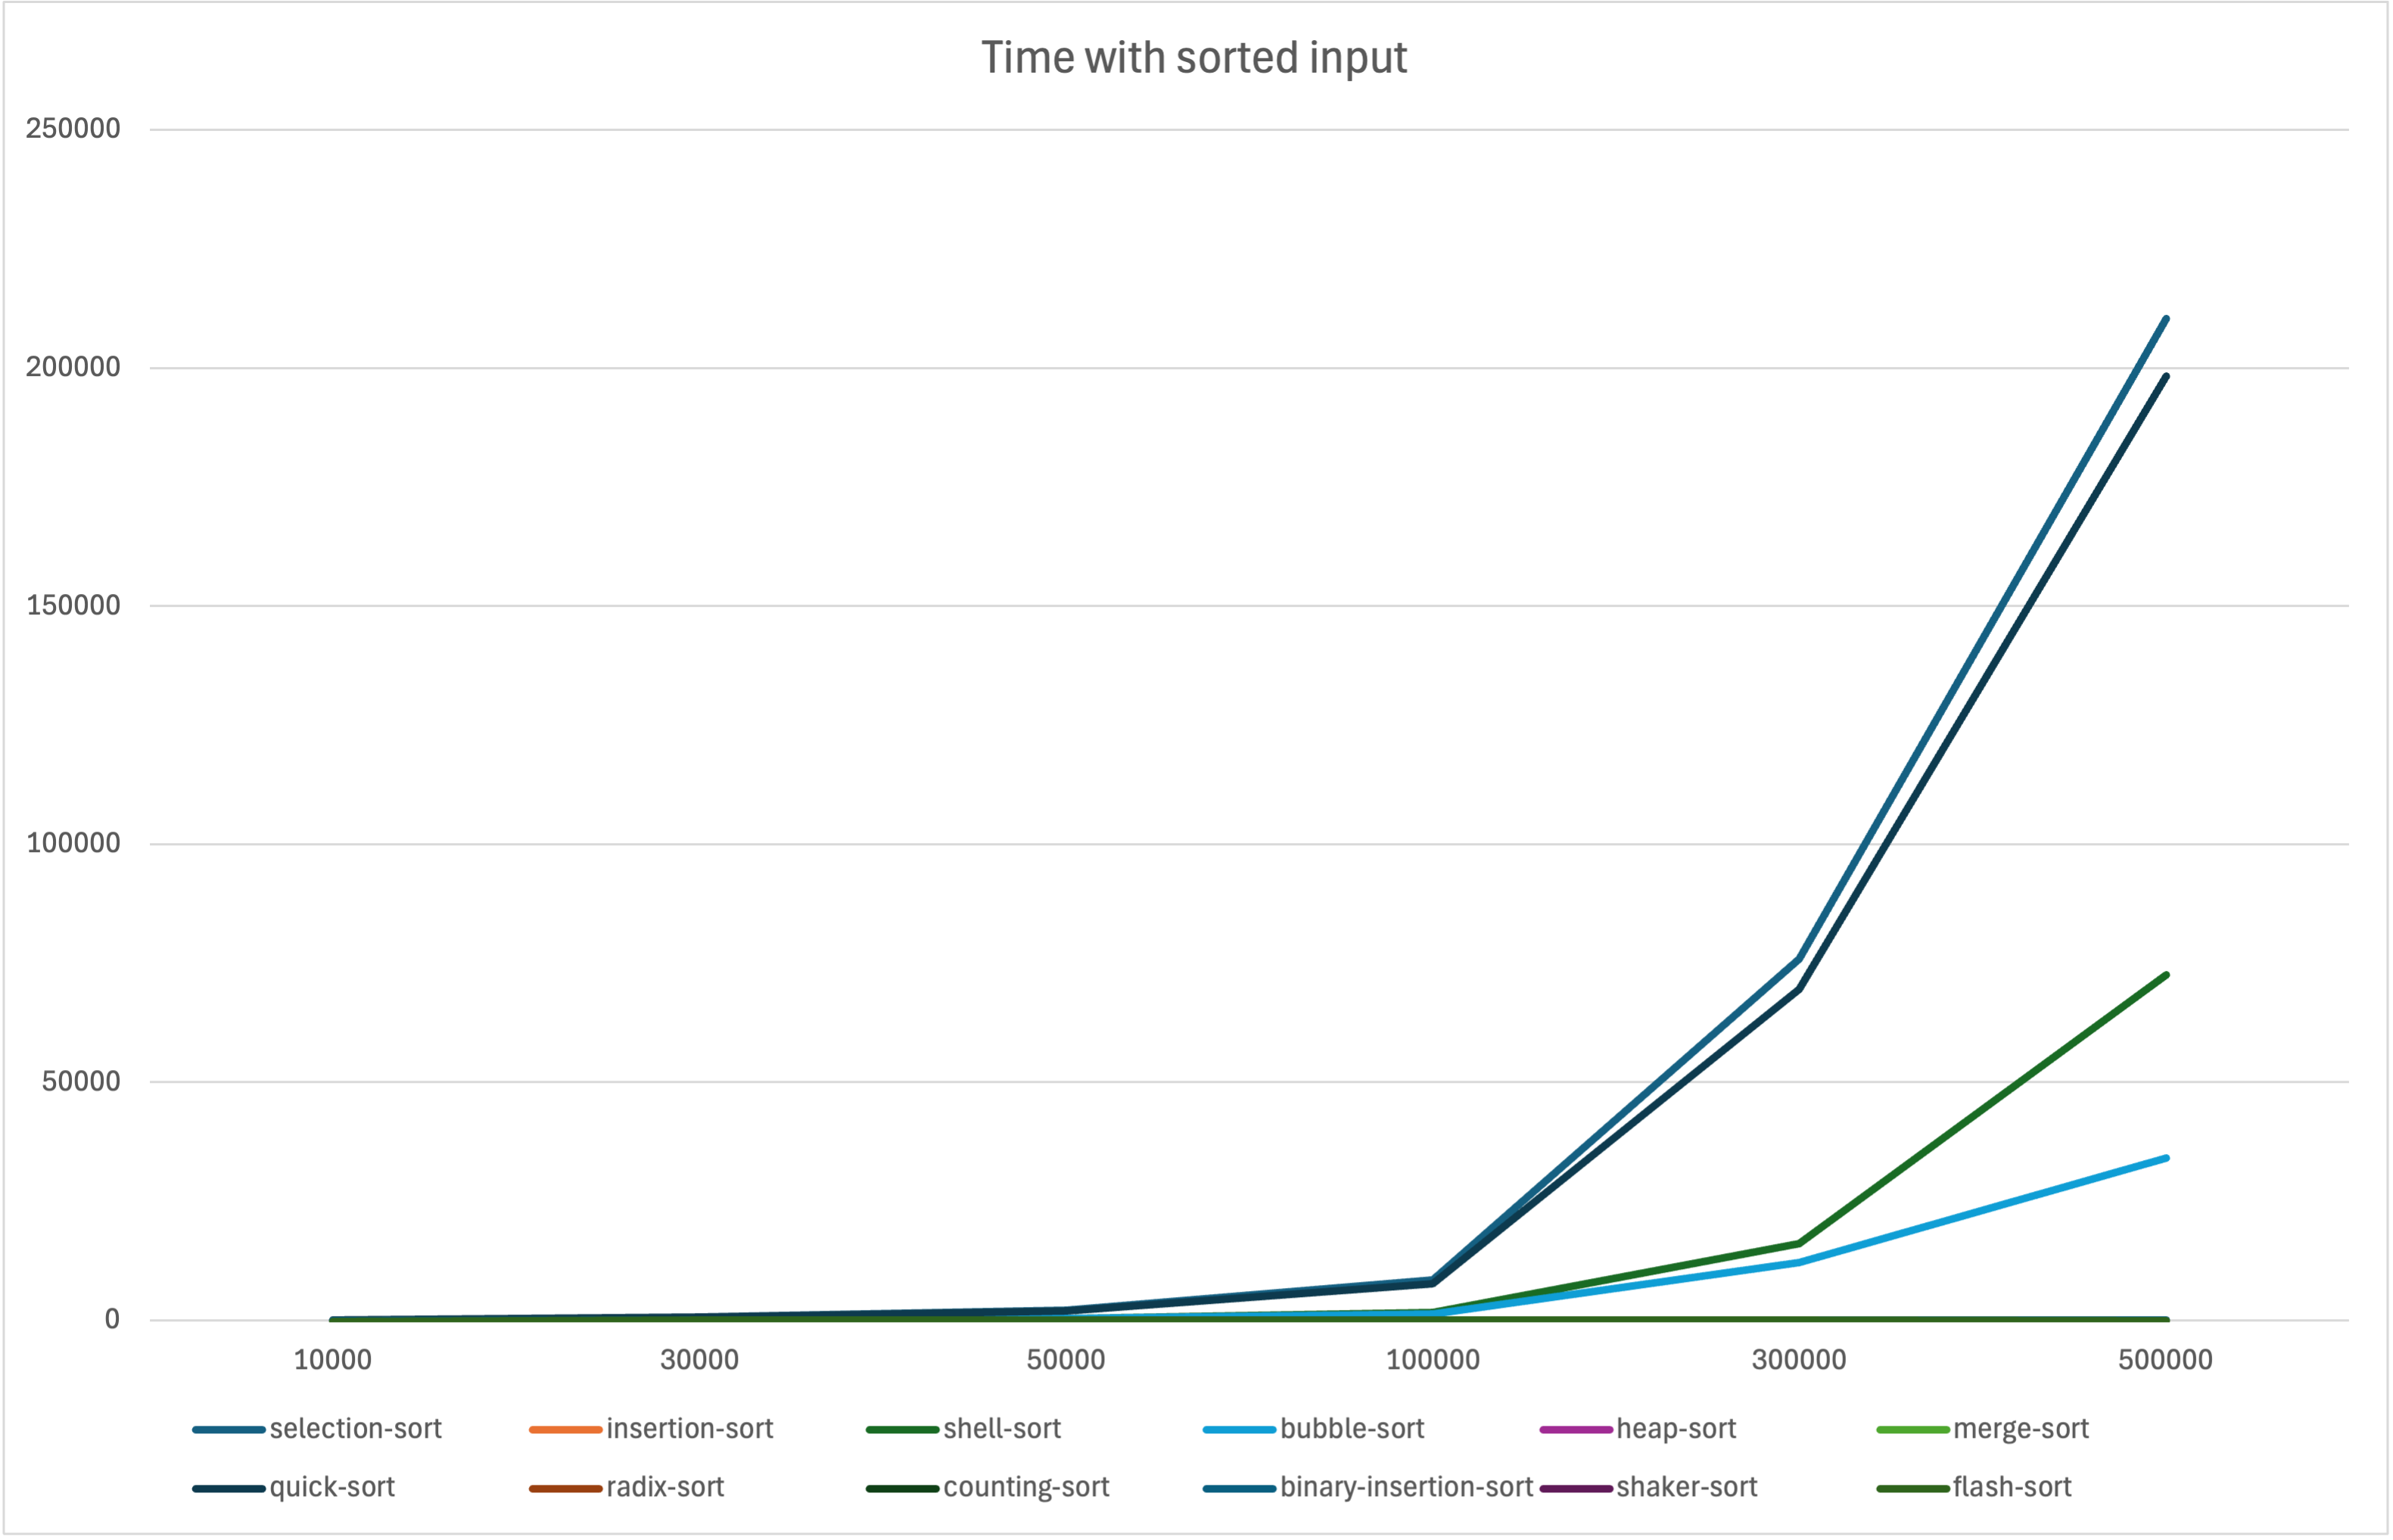
\includegraphics[scale=.65]{Figures/Visualization/Sorted_time.png}
    \caption{Execution time for Sorted data}
    \label{fig:enter-label}
\end{figure}

\textbf{Comments on the running time of sorting algorithms with sorted data}
\begin{enumerate}
    \item \textbf{Fastest Algorithms} \\
   - Insertion Sort: Extremely fast across all data sizes, maintaining very low execution times, which can be attributed to the sorted input allowing it to perform minimal operations. \\
   - Counting Sort and Radix Sort: Show low execution times, consistent with their linear or near-linear time complexity. \\
   - Flash Sort: Also performs well across different sizes, indicating efficiency in handling sorted data.

    \item \textbf{Slowest Algorithms} \\
   - Selection Sort: Performs poorly, with execution times increasing significantly with larger data sizes. This is due to its \(O(n^2)\) complexity. \\
   - Shell Sort and Bubble Sort: Have relatively high execution times, especially for larger data sizes, though they perform better than selection sort.

    \item \textbf{Moderate Performance} \\
   - Merge Sort, Heap Sort, Quick Sort: These algorithms show moderate execution times. Quick Sort's performance is likely impacted by pivot selection, which can lead to worse performance even on sorted input.
\end{enumerate}

\subsubsection{Comparison}

\vspace{5pt}

\begin{table}[h!]
\centering
\begin{tabular}{|l|r|r|r|r|r|r|}
\hline
\textbf{Algorithm} & \textbf{10000} & \textbf{30000} & \textbf{50000} & \textbf{100000} & \textbf{300000} & \textbf{500000} \\
\hline
Selection Sort & 100020001 & 900060001 & 2500100001 & 10000200001 & 90000600001 & 2.50001E+11 \\ \hline
Insertion Sort & 29998 & 89998 & 149998 & 299998 & 899998 & 1499998 \\ \hline
Shell Sort & 136486703 & 1228074234 & 3411144570 & 13643867417 & 1.2279E+11 & 3.41082E+11 \\ \hline
Bubble Sort & 100009999 & 900029999 & 2500049999 & 10000099999 & 90000299999 & 2.5E+11 \\ \hline
Heap Sort & 670329 & 2236648 & 3925351 & 8365080 & 27413230 & 47404886 \\ \hline
Merge Sort & 475242 & 1559914 & 2722826 & 5745658 & 18645946 & 32017850 \\ \hline
Quick Sort & 100019998 & 900059998 & 2500099998 & 10000199998 & 90000599998 & 2.50001E+11 \\ \hline
Radix Sort & 140051 & 510064 & 850064 & 1700064 & 6000077 & 10000777 \\ \hline
Counting Sort & 60003 & 180003 & 300003 & 600003 & 1800003 & 3000003 \\ \hline
Binary Insertion Sort & 370852 & 1251700 & 2203396 & 4706788 & 15527140 & 26927140 \\ \hline
Shaker Sort & 20002 & 60002 & 100002 & 200002 & 600002 & 1000002 \\ \hline
Flash Sort & 119000 & 357000 & 595000 & 1190000 & 3570000 & 5950000 \\
\hline
\end{tabular}
\label{table:number_of_comparisons}
\end{table}

\textbf{Comments on the number of comparisons of sorting algorithms with sorted data}
\begin{enumerate}
    \item \textbf{Fewest Comparisons} \\
   - Counting Sort: Performs the fewest comparisons as it is a non-comparison-based sort. \\
   - Insertion Sort: Very few comparisons are needed due to the already sorted input, similar to its execution time performance. \\
   - Flash Sort: Also shows low comparisons, consistent with its efficient performance.

    \item \textbf{Most Comparisons} \\
   - Shell Sort: Has an extremely high number of comparisons, especially at larger data sizes. \\
   - Bubble Sort: Also shows a high number of comparisons, though not as much as shell sort. \\
   - Selection Sort and Quick Sort: Both have high numbers of comparisons due to their \(O(n^2)\) and \(O(n\log n)\) complexities, respectively.
\end{enumerate}

\begin{figure}[h]
    \centering
    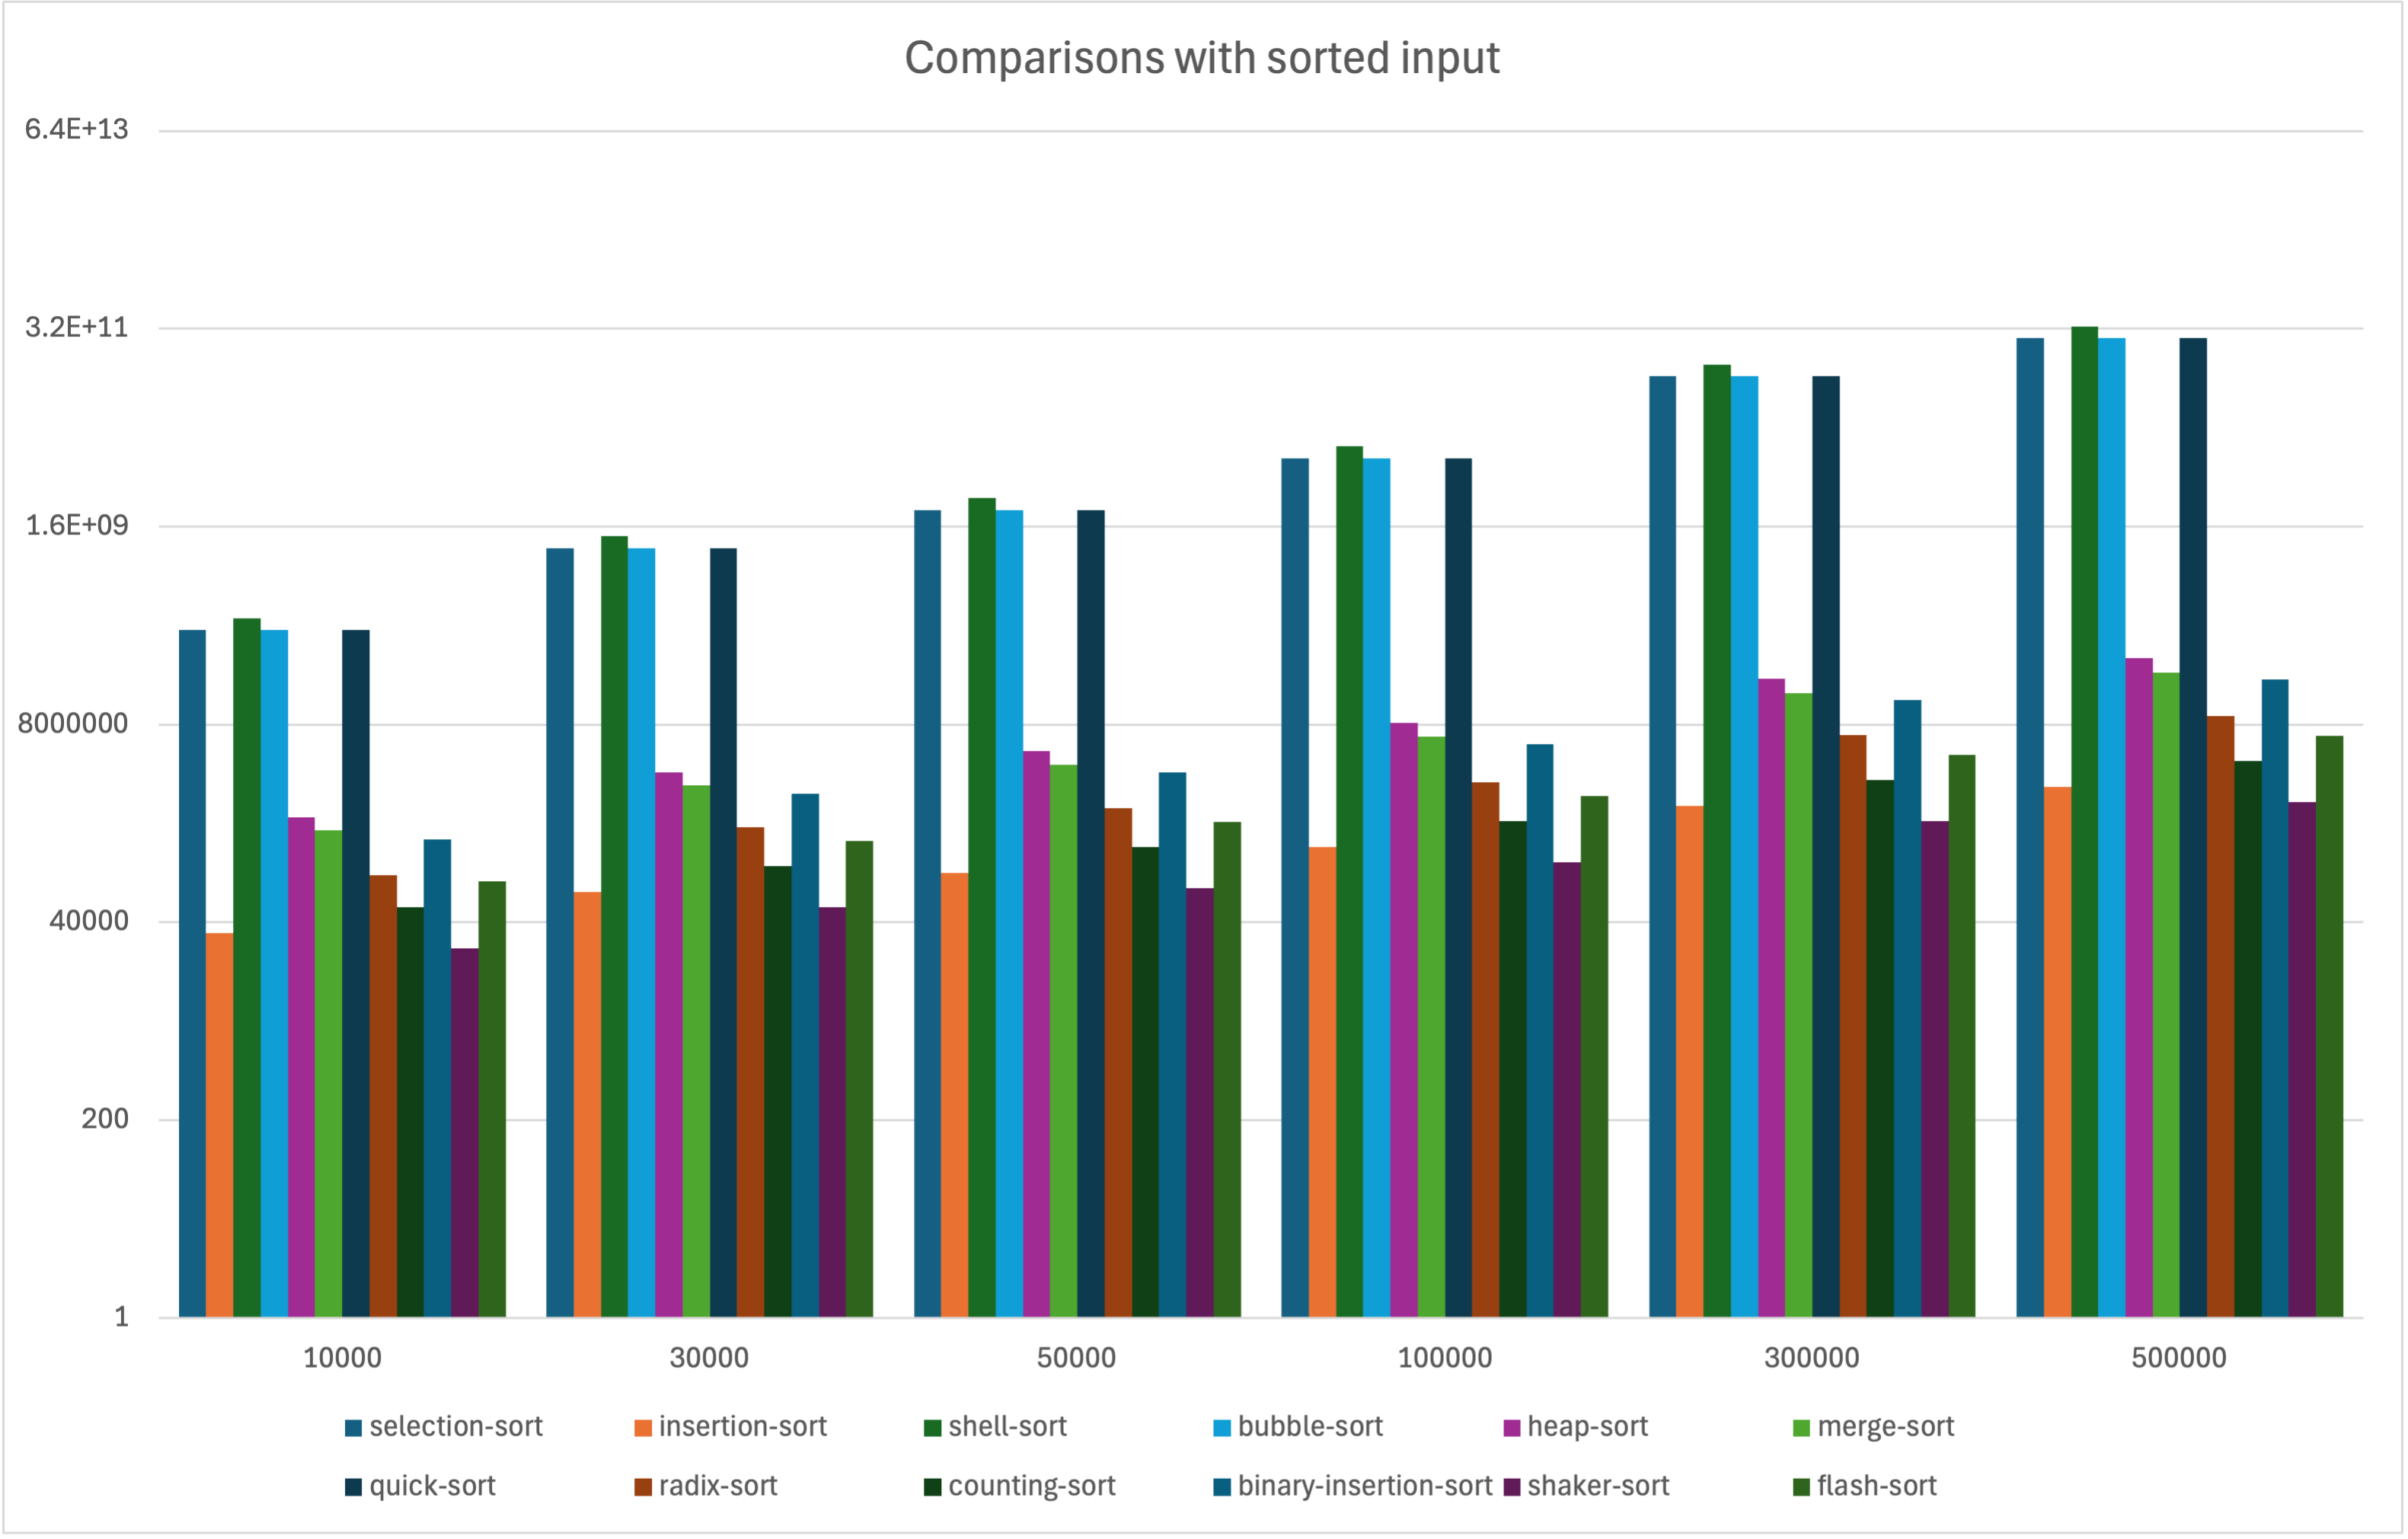
\includegraphics[scale=.65]{Figures/Visualization/Sorted_compare.png}
    \caption{Number of comparisons of the algorithm for Sorted data}
    \label{fig:enter-label}
\end{figure}

\newpage

\subsubsection{Overall}
\textbf{Overall comments on algorithms based on all data and size}
\begin{enumerate}
    \item \textbf{Data Order and Data Size} \\
   - For sorted data, insertion sort, counting sort, and flash sort are the best performers in terms of execution time and number of comparisons. \\
   - Selection sort, shell sort, and bubble sort are consistently the slowest and have the highest number of comparisons. \\
   - Merge sort, heap sort, and quick sort offer a balance but do not outperform the linear or near-linear algorithms for sorted data.

    \item \textbf{Stability:} \\
   - Stable Algorithms: Insertion sort, merge sort, and bubble sort are stable sorting algorithms. Insertion sort performs the best with sorted input among the stable sorts. \\
   - Unstable Algorithms: Quick sort, heap sort, and shell sort are unstable. Despite quick sort and heap sort being faster than shell sort in most cases, they are still outperformed by the linear time algorithms on sorted data.
\end{enumerate}


% \subsection{Reverse Data}
\subsubsection{Time}
\textbf{Comments on the running time of sorting algorithms with reverse data}
\begin{enumerate}
    \item \textbf{Fastest Algorithms:} \\
- \textit{Heap Sort}, \textit{Radix Sort}, and \textit{Counting Sort} again perform the fastest across all input sizes. Their execution times remain very low even for larger input sizes, similar to their performance on sorted input.

    \item \textbf{Slowest Algorithms:} \\
- \textit{Bubble Sort}, \textit{Shaker Sort}, and \textit{Quick Sort} exhibit very high execution times, especially as the input size increases. For instance, bubble sort's time grows from 76.9914 seconds at 10000 elements to 195572 seconds at 500000 elements.

    \item \textbf{Consistent Performers:} \\
- \textit{Merge Sort} and \textit{Shell Sort} show relatively stable and moderate execution times, indicating reliable performance across different input sizes.
\end{enumerate}

Execution time unit: milliseconds

\begin{table}[h!]
\centering
\begin{tabular}{|l|r|r|r|r|r|r|}
\hline
\textbf{Algorithm} & \textbf{10000} & \textbf{30000} & \textbf{50000} & \textbf{100000} & \textbf{300000} & \textbf{500000} \\
\hline
Selection Sort & 85.285 & 764.617 & 2085.39 & 8471.83 & 75944.1 & 210673 \\ \hline
Insertion Sort & 11.1563 & 100.834 & 276.323 & 1090.38 & 9847.49 & 28014.6 \\ \hline
Shell Sort & 21.0003 & 203.454 & 527.093 & 2115.4 & 18846.1 & 55537.9 \\ \hline
Bubble Sort & 76.9914 & 692.504 & 1928.01 & 7667.36 & 69228.6 & 195572 \\ \hline
Heap Sort & 0.6743 & 2.2238 & 4.1879 & 8.3122 & 26.5599 & 45.5919 \\ \hline
Merge Sort & 2.5089 & 7.4184 & 12.1534 & 23.8237 & 73.346 & 123.387 \\ \hline
Quick Sort & 44.9166 & 400.345 & 1098.21 & 4412.2 & 39600.2 & 112705 \\ \hline
Radix Sort & 0.133 & 0.4967 & 0.8283 & 1.5792 & 5.9777 & 10.3353 \\ \hline
Counting Sort & 0.016 & 0.0421 & 0.0752 & 0.1617 & 0.6948 & 1.2085 \\ \hline
Binary Insertion Sort & 7.9368 & 78.3401 & 204.501 & 795.454 & 7076.07 & 21493.8 \\ \hline
Shaker Sort & 81.9425 & 730.12 & 2068.47 & 8181.6 & 73751.9 & 204937 \\ \hline
Flash Sort & 0.1018 & 0.317 & 0.6843 & 1.3254 & 3.8055 & 6.2582 \\
\hline
\end{tabular}
\label{table:reverse_execution_time}
\end{table}

\begin{figure}[h]
    \centering
    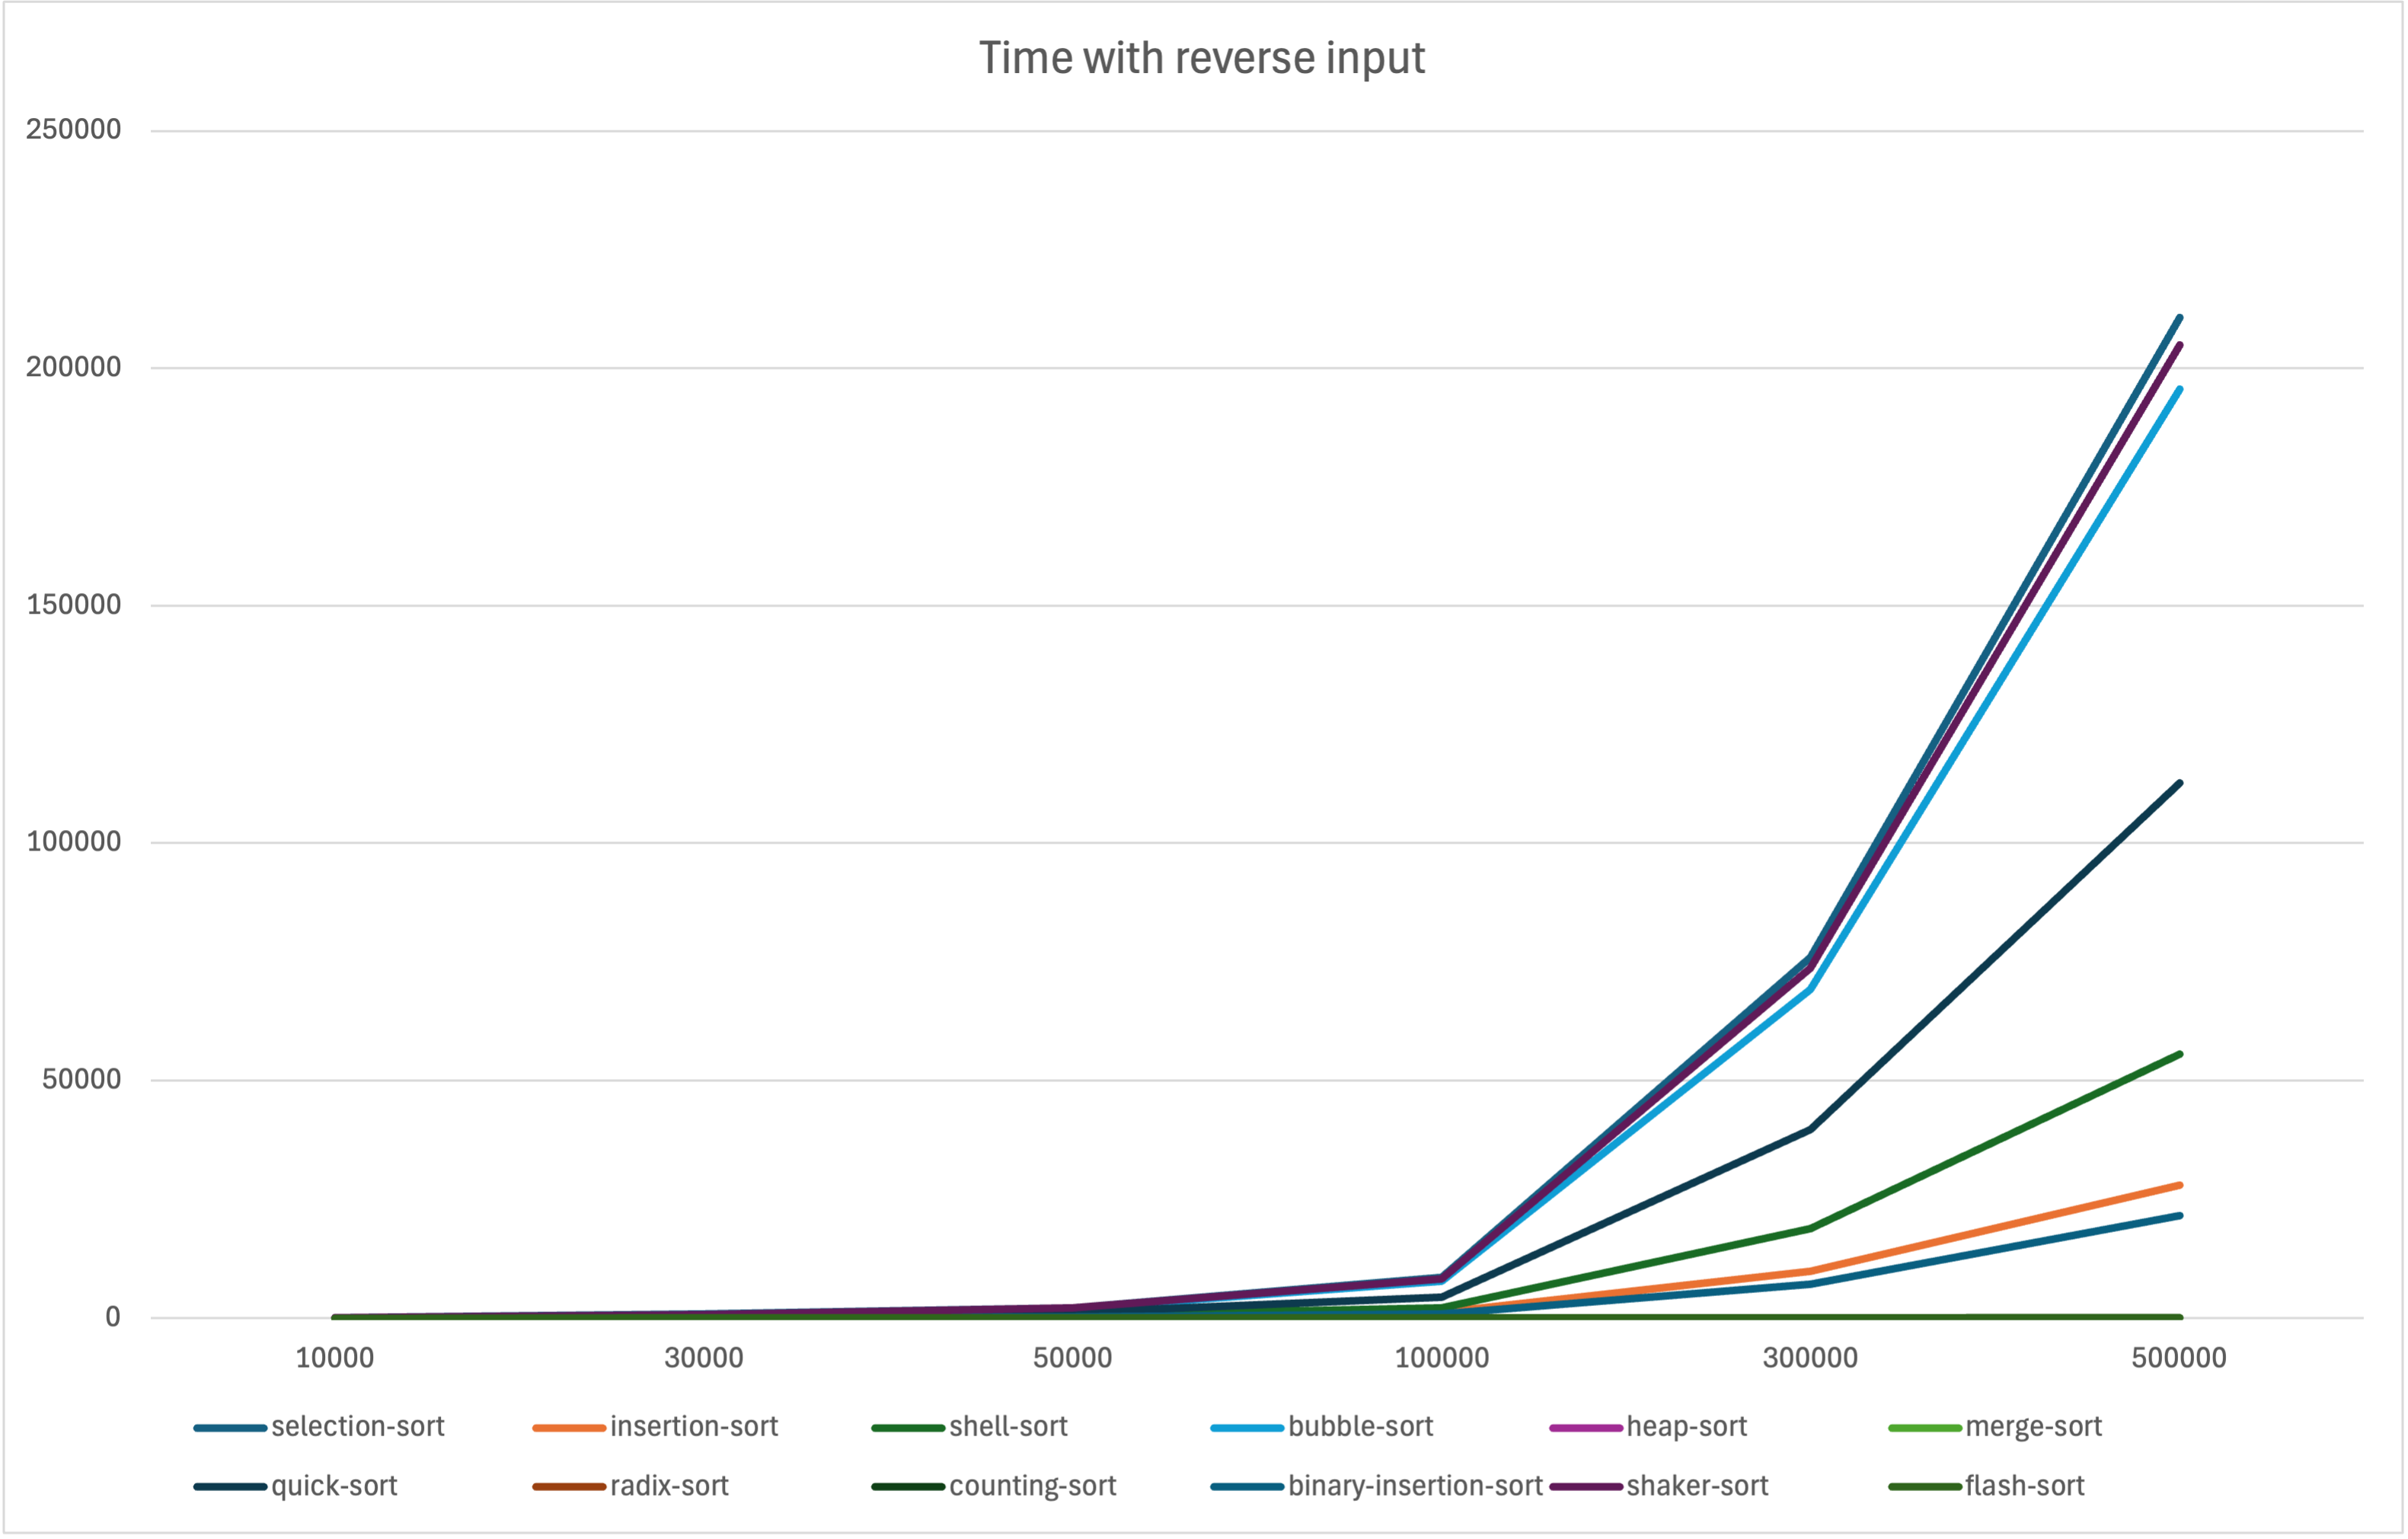
\includegraphics[scale=.65]{Figures/Visualization/Reverse_time.png}
    \caption{Execution time for Reverse data}
    \label{fig:enter-label}
\end{figure}

\subsubsection{Comparison}

\textbf{Comments on the number of comparisons of sorting algorithms with reverse data}
\begin{enumerate}
    \item \textbf{Fewest Comparisons:} \\
- \textit{Counting Sort} and \textit{Radix Sort} consistently perform the fewest comparisons, highlighting their efficiency in this metric for reverse sorted inputs as well.

    \item \textbf{Most Comparisons:} \\
- \textit{Selection Sort}, \textit{Insertion Sort}, \textit{Bubble Sort}, and \textit{Quick Sort} show an extremely high number of comparisons, reaching up to the order of \(10^{11}\) for larger input sizes, indicating significant inefficiency in terms of comparisons.

    \item \textbf{Consistent Performers:} \\
- \textit{Heap Sort}, \textit{Merge Sort}, and \textit{Binary Insertion Sort} maintain a moderate and steadily increasing number of comparisons, showing balanced performance.
\end{enumerate}

\begin{table}[h!]
\centering
\begin{tabular}{|l|r|r|r|r|r|r|}
\hline
\textbf{Algorithm} & \textbf{10000} & \textbf{30000} & \textbf{50000} & \textbf{100000} & \textbf{300000} & \textbf{500000} \\
\hline
Selection Sort & 100020001 & 900060001 & 2500100001 & 10000200001 & 90000600001 & 2.50001E+11 \\ \hline
Insertion Sort & 100009999 & 900029999 & 2500049999 & 10000099999 & 90000299999 & 2.5E+11 \\ \hline
Shell Sort & 136486703 & 1228074234 & 3411144570 & 13643867417 & 1.2279E+11 & 3.41082E+11 \\ \hline
Bubble Sort & 100009999 & 900029999 & 2500049999 & 10000099999 & 90000299999 & 2.5E+11 \\ \hline
Heap Sort & 606771 & 2063324 & 3612724 & 7718943 & 25569379 & 44483348 \\ \hline
Merge Sort & 476441 & 1573465 & 2733945 & 5767897 & 18708313 & 32336409 \\ \hline
Quick Sort & 100019998 & 900059998 & 2500099998 & 10000199998 & 90000599998 & 2.50001E+11 \\ \hline
Radix Sort & 140051 & 510064 & 850064 & 1700064 & 6000077 & 10000077 \\ \hline
Counting Sort & 60003 & 180003 & 300003 & 600003 & 1800003 & 3000003 \\ \hline
Binary Insertion Sort & 50348179 & 451187593 & 1252080140 & 5004460231 & 45014870410 & 1.25026E+11 \\ \hline
Shaker Sort & 100005001 & 900015001 & 2500025001 & 10000050001 & 90000150001 & 2.5E+11 \\ \hline
Flash Sort & 103753 & 311253 & 518753 & 1037503 & 3112503 & 5187503 \\
\hline
\end{tabular}
\label{table:reverse_number_of_comparisons}
\end{table}

\begin{figure}[h]
    \centering
    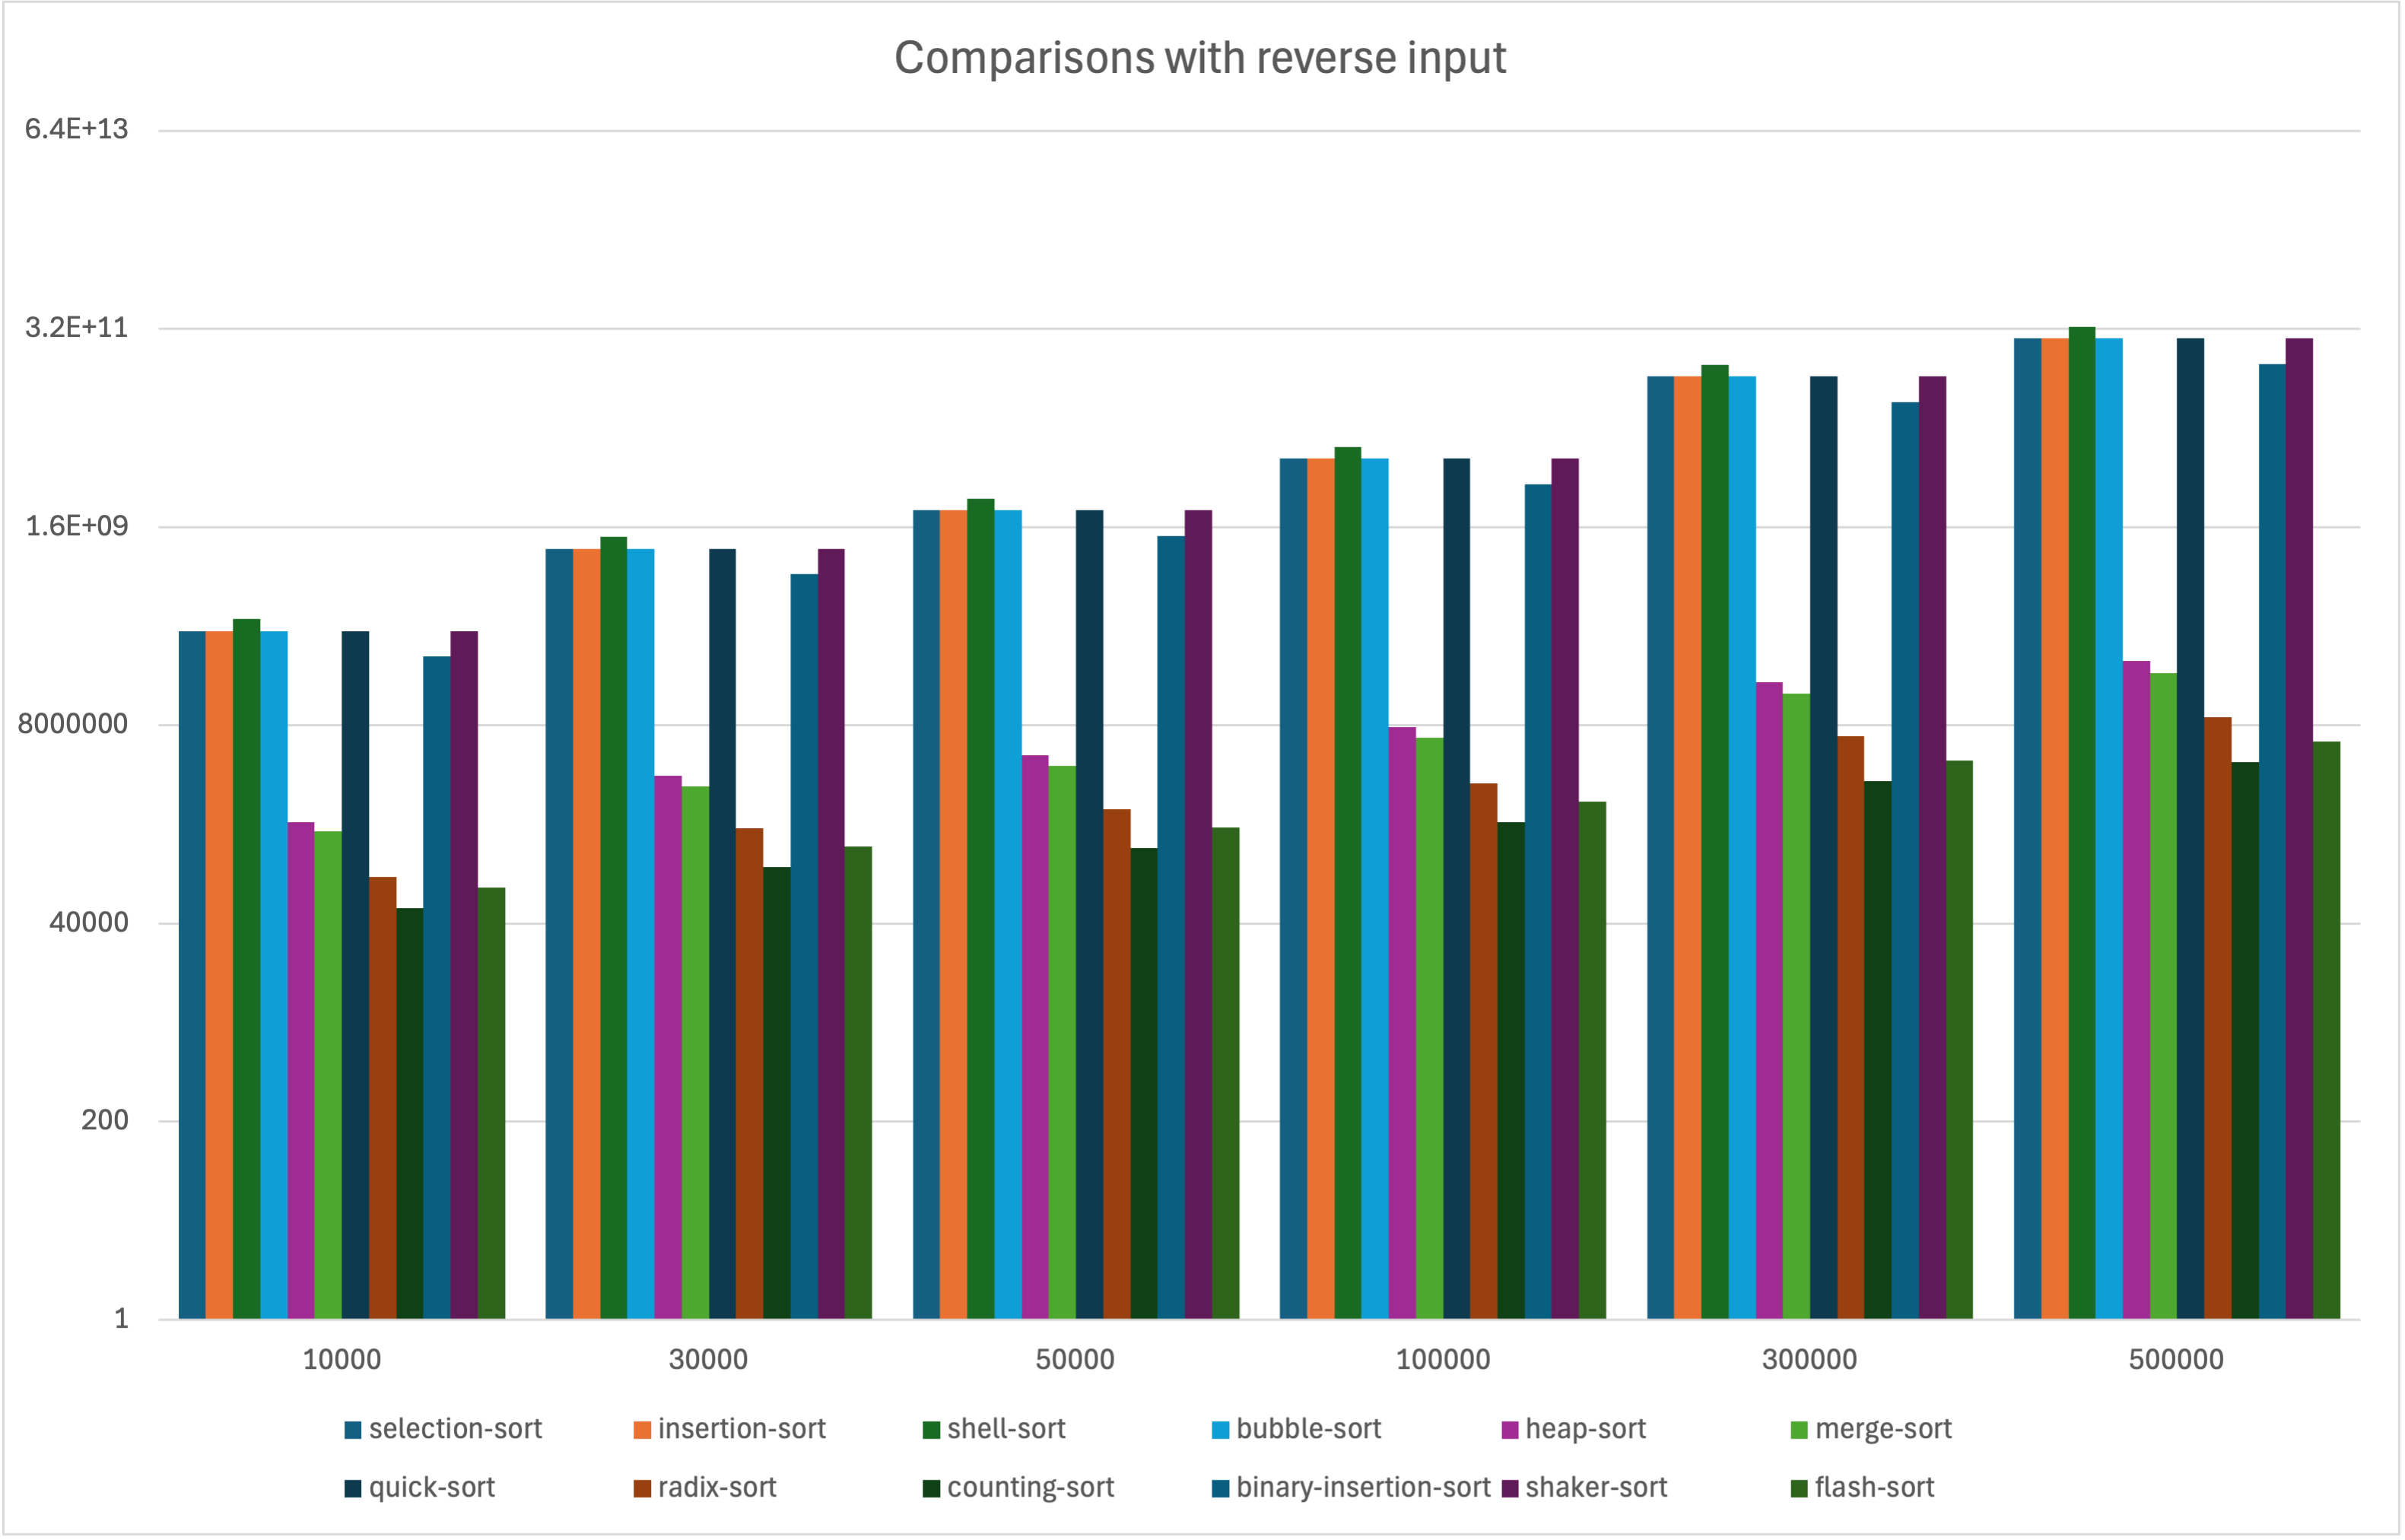
\includegraphics[scale=.65]{Figures/Visualization/Reverse_compare.png}
    \caption{Number of comparisons of the algorithm for Reverse data}
    \label{fig:enter-label}
\end{figure}

\subsubsection{Overall}
\begin{enumerate}
    \item \textbf{Stable Algorithms:} \\
- \textit{Heap Sort}, \textit{Radix Sort}, and \textit{Merge Sort} are stable across both sorted and reverse sorted data in terms of execution time and number of comparisons. These algorithms are generally reliable and efficient.

    \item \textbf{Unstable Algorithms:} \\
- \textit{Quick Sort}, \textit{Selection Sort}, \textit{Bubble Sort}, and \textit{Shaker Sort} are unstable, especially with a significant increase in execution time and number of comparisons as the input size grows. These algorithms tend to be inefficient for larger datasets and in different data orders.

    \item \textbf{Fastest Algorithms Overall:} \\
- \textit{Insertion Sort}, \textit{Counting Sort}, and \textit{Binary Insertion Sort} consistently show the fastest execution times, particularly for smaller input sizes. Their performance is highly efficient for both sorted and reverse sorted inputs.

    \item \textbf{Slowest Algorithms Overall:} \\
- \textit{Selection Sort}, \textit{Bubble Sort}, and \textit{Shaker Sort} are the slowest overall, showing significantly higher execution times and a very high number of comparisons for larger datasets and different data orders.
\end{enumerate}

% \subsection{Nearly Sorted Data}
\subsubsection{Time}
Execution time unit: milliseconds
\begin{table}[h!]
\centering
\begin{tabular}{|l|r|r|r|r|r|r|}
\hline
\textbf{Algorithm} & \textbf{10000} & \textbf{30000} & \textbf{50000} & \textbf{100000} & \textbf{300000} & \textbf{500000} \\
\hline
Selection Sort & 83.898 & 754.469 & 2097.2 & 8461.66 & 76561.9 & 210139 \\ \hline
Insertion Sort & 0.02 & 0.0912 & 0.0799 & 0.1037 & 0.1879 & 0.3103 \\ \hline
Shell Sort & 20.4246 & 195.299 & 484.834 & 1795.67 & 15977.1 & 49089.4 \\ \hline
Bubble Sort & 14.3526 & 124.481 & 347.676 & 1339.36 & 12296.1 & 34055 \\ \hline
Heap Sort & 0.6889 & 2.3363 & 3.8533 & 8.278 & 29.1528 & 43.6957 \\ \hline
Merge Sort & 2.497 & 8.2457 & 12.1077 & 27.873 & 72.59 & 120.094 \\ \hline
Quick Sort & 19.2834 & 152.439 & 1281.55 & 7068.34 & 68668.4 & 197042 \\ \hline
Radix Sort & 0.1272 & 0.5591 & 0.8446 & 1.5646 & 5.8751 & 10.27 \\ \hline
Counting Sort & 0.0155 & 0.043 & 0.0714 & 0.1567 & 0.7502 & 1.4829 \\ \hline
Binary Insertion Sort & 0.271 & 0.9111 & 1.4968 & 3.1023 & 9.2867 & 16.3849 \\ \hline
Shaker Sort & 0.1591 & 0.3401 & 0.2698 & 0.327 & 0.3967 & 0.5661 \\ \hline
Flash Sort & 0.0961 & 0.3437 & 0.6098 & 0.992 & 4.0775 & 6.7901 \\
\hline
\end{tabular}
\label{table:nearly_sorted_execution_time}
\end{table}

\begin{figure}[h]
    \centering
    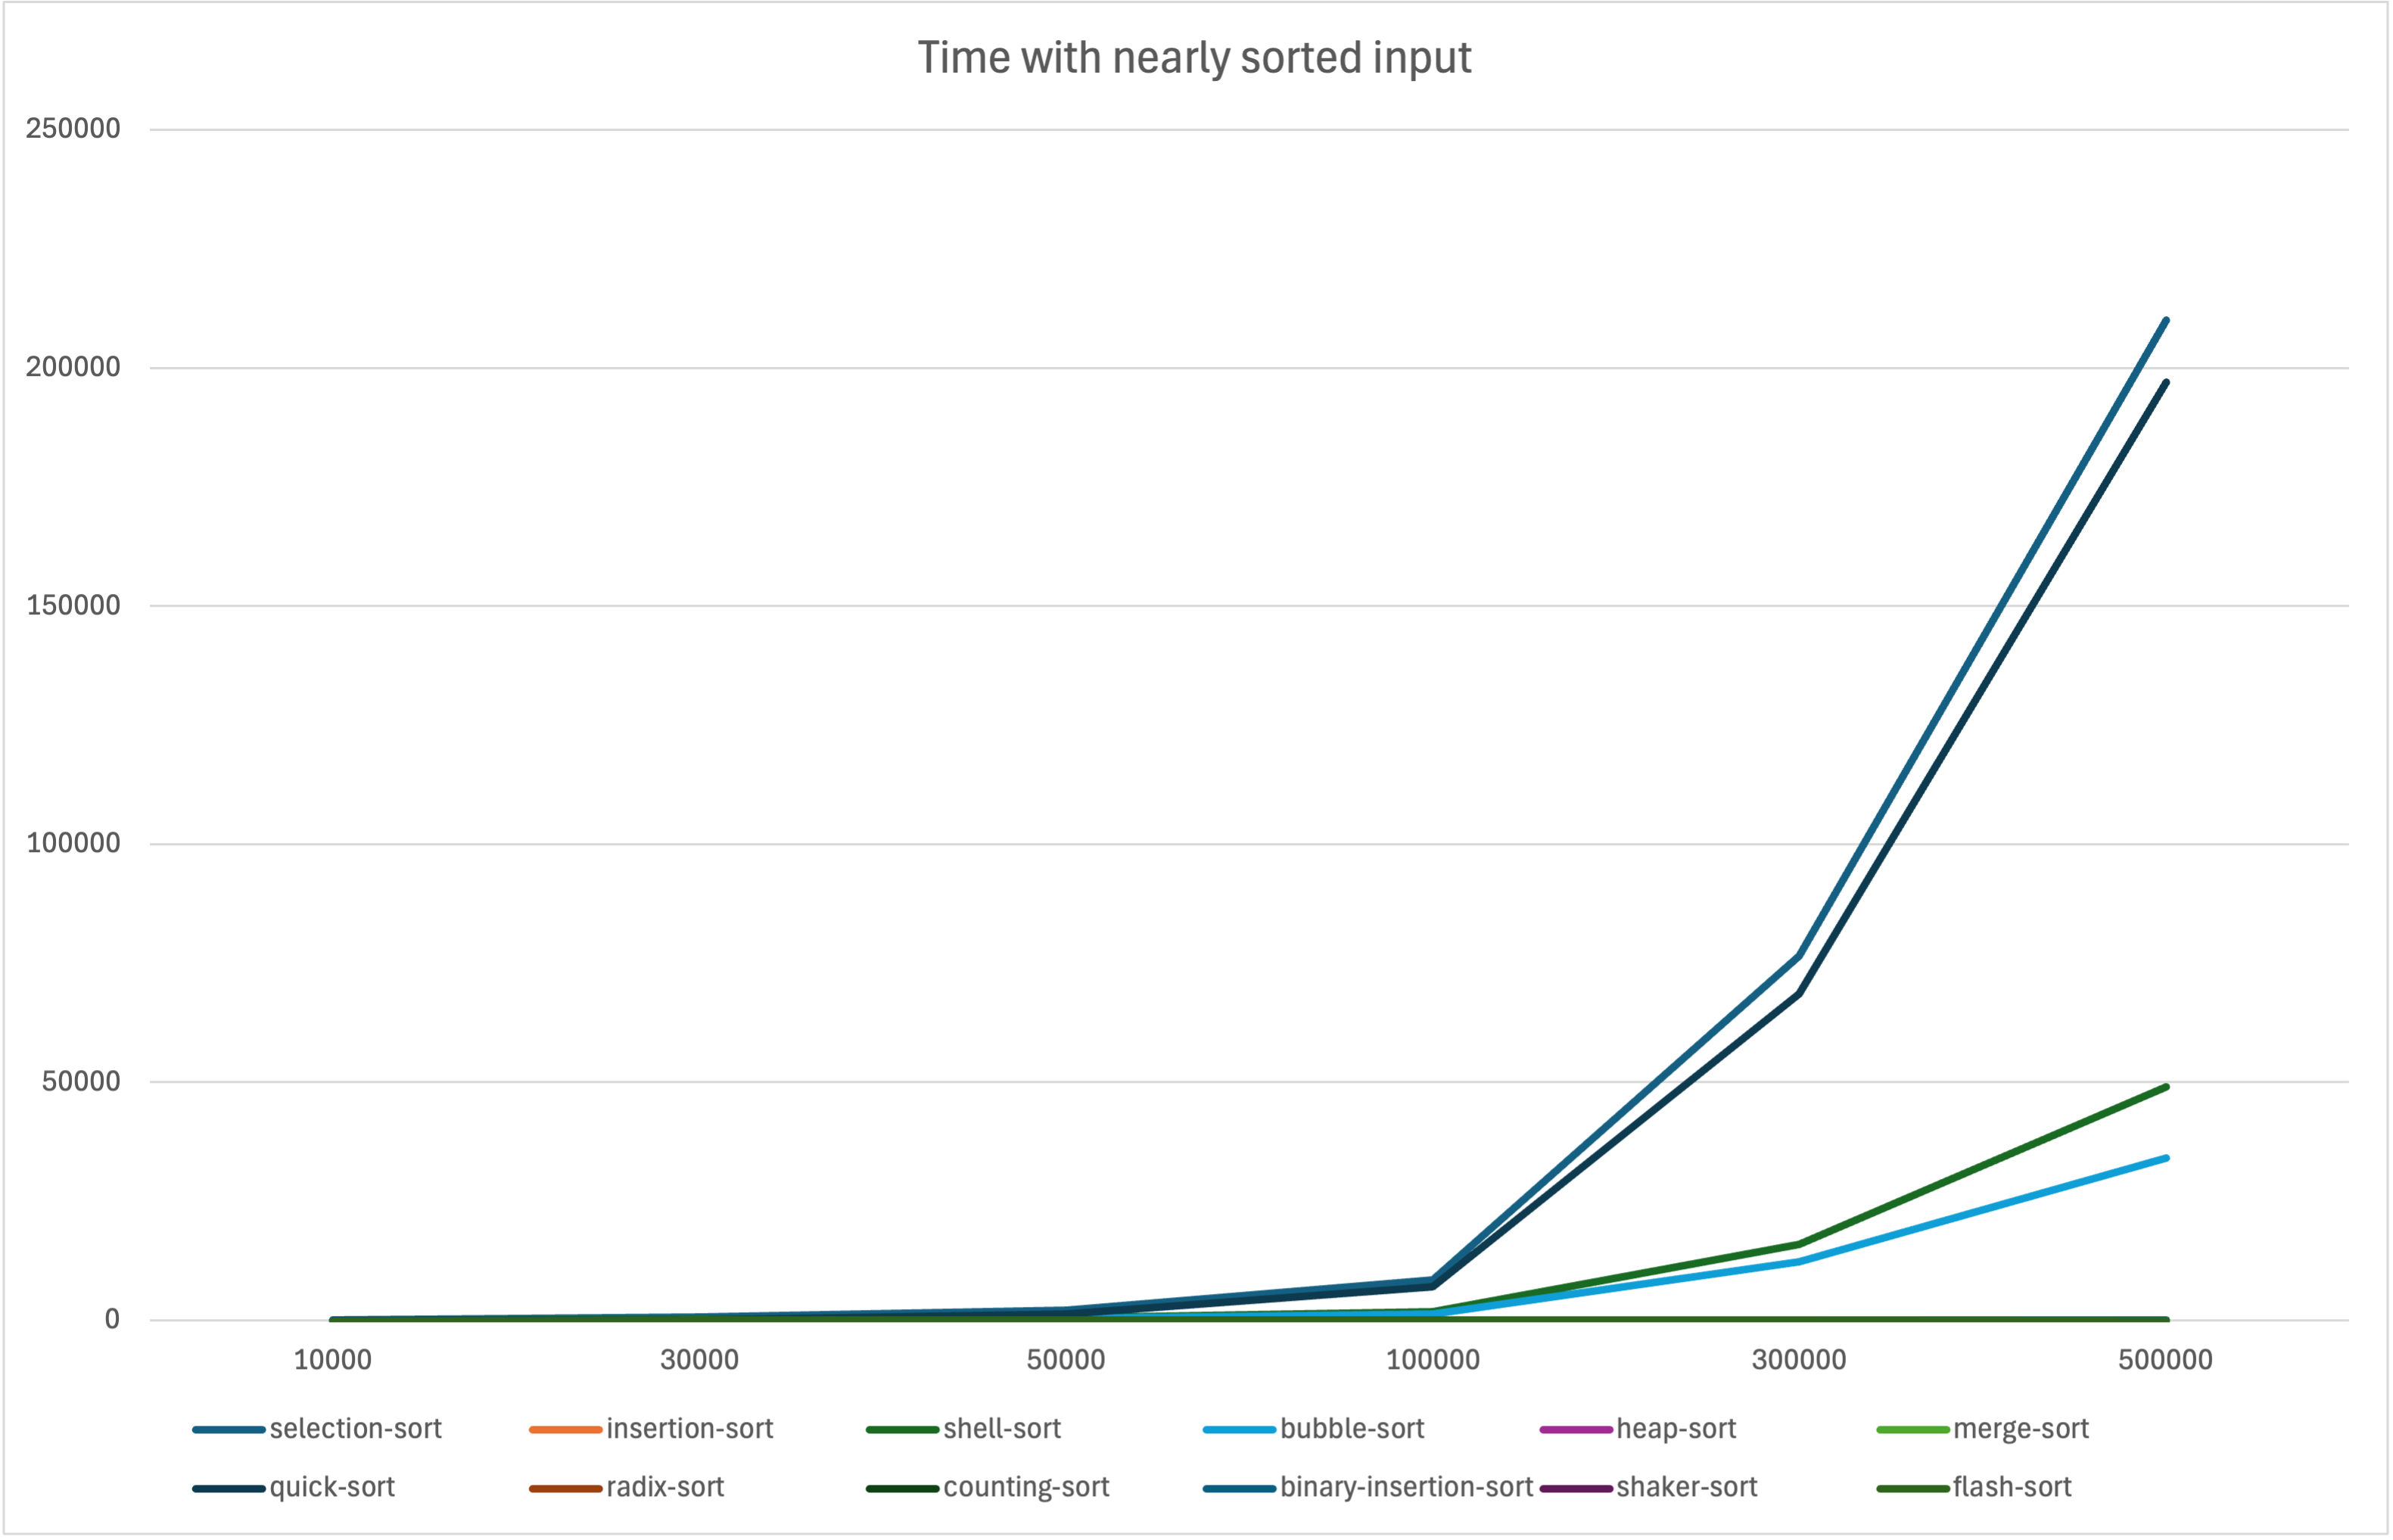
\includegraphics[scale=.65]{Figures/Visualization/Nearly_time.png}
    \caption{Execution time for Nearly Sorted data}
    \label{fig:enter-label}
\end{figure}

\textbf{Comments on the running time of sorting algorithms with nearly sorted data}

\begin{enumerate}
    \item \textbf{Fastest Algorithm:} \\
  - For small data sizes (10,000 - 50,000), \textit{Insertion Sort} has the fastest execution time. \\
  - As data size increases (100,000 - 500,000), \textit{Counting Sort} and \textit{Flash Sort} become the most efficient in terms of execution time.

    \item \textbf{Slowest Algorithm:}
  - \textit{Selection Sort} and \textit{Bubble Sort} are the slowest algorithms for all data sizes.

    \item \textbf{General Comments:}
  - Algorithms like \textit{Quick Sort}, \textit{Merge Sort}, and \textit{Heap Sort} have moderate execution times, better than \textit{Selection Sort} and \textit{Bubble Sort}, but slower than \textit{Counting Sort} and \textit{Flash Sort}.
\end{enumerate}


\subsubsection{Comparison}
\begin{table}[h!]
\centering
\begin{tabular}{|l|r|r|r|r|r|r|}
\hline
\textbf{Algorithm} & \textbf{10000} & \textbf{30000} & \textbf{50000} & \textbf{100000} & \textbf{300000} & \textbf{500000} \\
\hline
Selection Sort & 100020001 & 900060001 & 2500100001 & 10000200001 & 90000600001 & 2.50001E+11 \\ \hline
Insertion Sort & 147654 & 744478 & 651114 & 801114 & 1401114 & 2069258 \\ \hline
Shell Sort & 136486703 & 1228074234 & 3411144570 & 13643867417 & 1.2279E+11 & 3.41082E+11 \\ \hline
Bubble Sort & 100009999 & 900029999 & 2500049999 & 10000099999 & 90000299999 & 2.5E+11 \\ \hline
Heap Sort & 669993 & 2236691 & 3925392 & 8364913 & 27413230 & 47404908 \\ \hline
Merge Sort & 507409 & 1666255 & 2833852 & 5856684 & 18744620 & 32121800 \\ \hline
Quick Sort & 29623224 & 252918102 & 1706786888 & 9235419190 & 89219734904 & 2.49335E+11 \\ \hline
Radix Sort & 140051 & 510064 & 850064 & 1700064 & 6000077 & 10000077 \\ \hline
Counting Sort & 60003 & 180003 & 300003 & 600003 & 1800003 & 3000003 \\ \hline
Binary Insertion Sort & 437075 & 1467163 & 2451861 & 4879730 & 15700082 & 27071229 \\ \hline
Shaker Sort & 183347 & 474192 & 465899 & 565899 & 965899 & 1475760 \\ \hline
Flash Sort & 118975 & 356977 & 594976 & 1189973 & 3569971 & 5949978 \\
\hline
\end{tabular}
\label{table:nearly_sorted_number_of_comparisons}
\end{table}

\begin{figure}[h]
    \centering
    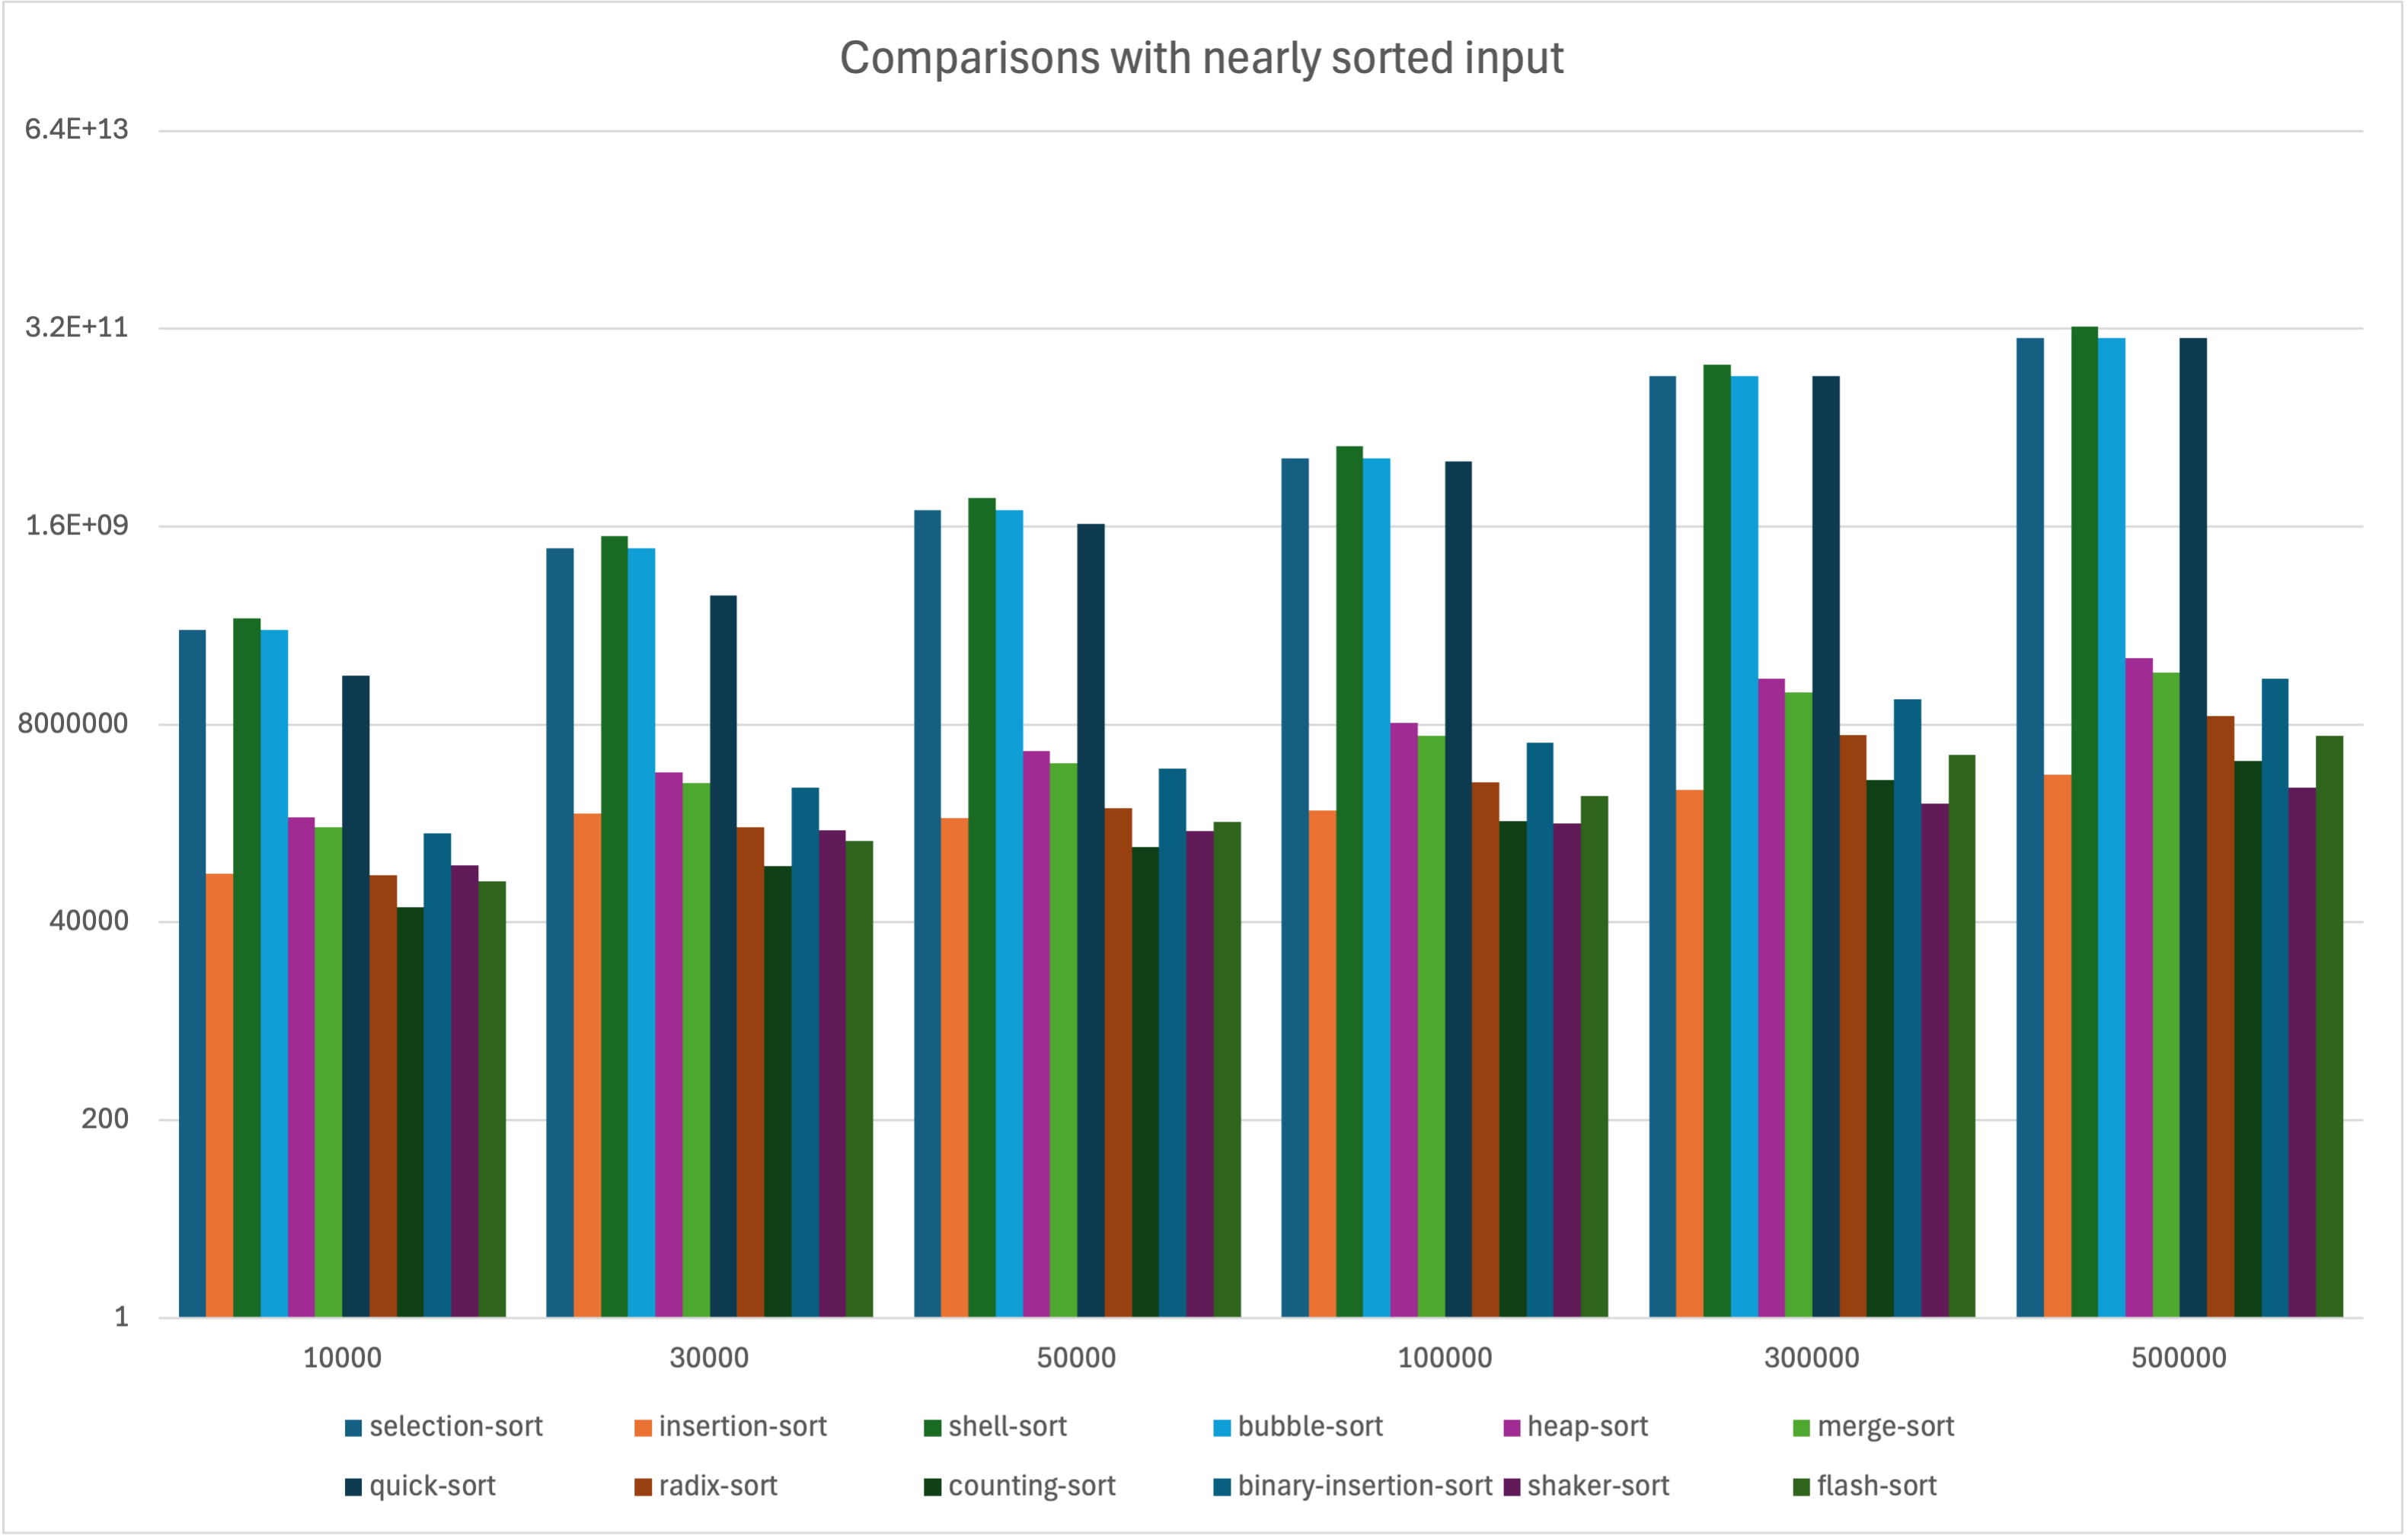
\includegraphics[scale=.65]{Figures/Visualization/Nearly_compare.png}
    \caption{Number of comparisons of the algorithm for Nearly Sorted data}
    \label{fig:enter-label}
\end{figure}

\textbf{Comments on the number of comparisons of sorting algorithms with nearly sorted data}

\begin{enumerate}
    \item \textbf{Algorithm with Fewest Comparisons:} \\
  - \textit{Counting Sort} and \textit{Radix Sort} have the fewest comparisons for all data sizes.

    \item \textbf{Algorithm with Most Comparisons:}
  - \textit{Selection Sort}, \textit{Bubble Sort}, and \textit{Shell Sort} have the most comparisons for all data sizes.

    \item \textbf{General Comments:} \\
  - Algorithms like \textit{Merge Sort} and \textit{Heap Sort} have relatively fewer comparisons compared to \textit{Selection Sort} and \textit{Bubble Sort}.
\end{enumerate}

\subsubsection{Overall}
\begin{enumerate}
    \item \textbf{By Data Order:}
    \begin{itemize}[label=-]
        \item  \textit{Insertion Sort} performs best when the data is nearly sorted.
        \item \textit{Selection Sort} and \textit{Bubble Sort} remain slow and inefficient with nearly sorted data.
    \end{itemize}
    
    \item \textbf{By Data Size:}
    \begin{itemize}[label=-]
        \item  For small data sizes, \textit{Insertion Sort} and \textit{Counting Sort} have the best execution times.
        \item  For large data sizes, \textit{Counting Sort} and \textit{Flash Sort} excel in execution time.
        \item \textit{Quick Sort} and \textit{Merge Sort} can be considered good choices for medium to large data sizes due to their balance between execution time and comparison count.
    \end{itemize}
    
    \item \textbf{Grouping Stable/Unstable Algorithms:}
    \begin{itemize}[label=-]
        \item  \textbf{Stable:} \\
  - \textit{Insertion Sort}, \textit{Merge Sort}, and \textit{Binary Insertion Sort} are stable algorithms, ensuring the order of equal elements is preserved.
  
        \item  \textbf{Unstable:} \\
  - \textit{Quick Sort}, \textit{Heap Sort}, and \textit{Shell Sort} are unstable algorithms and may change the order of equal elements.
    \end{itemize}
\end{enumerate}
% \newpage

% \section{Project Organization and Programming Note}
% All source codes are located in "SOURCE" folder.
% \subsection{Project organization}
\begin{enumerate}
    \item Header files
    \begin{itemize}[label=-]
        \item SortWithTime.h: This file contains the declaration of all original sorting algorithms which are used to measure the time of each algorithm.
        \item SortWithComapre.h: This file contains the declaration of all sorting algorithms which are used to counting the number of comparisons of each algorithm.
        \item CommandLine.h: This file contains the declarations of below things:
        \begin{itemize}
            \item Declare all commands  which can be used when executing the file exe
            \item Declare necessary functions to run the commands.
        \end{itemize}

        \item DataGenerator.h: This file contains the below things:
        \begin{itemize}
            \item Declare the functions to generate data in different orders and different sizes.
            \item Declare the functions to read files to get data and write data into files.
            \item Declare the function to duplicate an array.
            \item Declare the functions to measure the time and counting the comparison of given algorithm.
            \item The given template and given function for the template.
        \end{itemize}
        \item Lib.h: This file contains all the necessary libraries.
    \end{itemize}
    \item .cpp files
    \begin{itemize}[label=-]
        \item The cpp files in folder contains all definitions of the functions that are declared in the header files. "main.cpp" contains the \texttt{main()} function.
    \end{itemize}
    \item Generative Text files
    \begin{itemize}[label=-]
        \item There are 5 input text files and 1 output text files which is created when running the commands. 
    \end{itemize}
\end{enumerate}
\textbf{NOTE:} Using these text files is optional, and alternatively, you can create new files in this format.

% \subsection{Programming note}
Chrono library: use for measuring running time of sorting functions
\begin{itemize}[label=-]
    \item \texttt{<chrono>} is a \texttt{C++} header that provides a collection of types and functions to work with time. It is a part of the \texttt{C++} Standard Template Library (STL) and it’s included in \texttt{C++11} and later versions. ~\cite{ref13}
    \item \texttt{<chrono>} provides three main types of clocks: 
        \begin{itemize}[label=$\bullet$]
            \item \texttt{system\_clock}, \texttt{steady\_clock}, and \texttt{high\_resolution\_clock}. 
            
            \item These clocks are used to measure time in various ways. ~\cite{ref13}
        \end{itemize}
    \item Here is a pseudocode:
        \begin{itemize}[label=$\bullet$]
            \item \texttt{start\_time = get\_current\_high\_resolution\_time()} (record the current time)
            
            \item \texttt{runSortingAlgorithmWithTime(a, n, algoIndex)} (calling function)
            
            \item \texttt{end\_time = get\_current\_high\_resolution\_time()} (record the current time)
            
            \item \texttt{duration = end\_time - start\_time} (calculate the duration in milliseconds)
            
            \item \texttt{time = convert\_to\_milliseconds(duration)} (convert duration to milliseconds)
        \end{itemize}
\end{itemize}

% \newpage

% \section{How to compile}
% To compile this project, follow the steps below:
\begin{enumerate}
    \item Ensure you have a \texttt{C++} compiler installed on your system. Common options include \texttt{g++} (\texttt{std=c++11} or later) and \texttt{clang++}.
    \item Open a terminal and navigate to the directory containing the project's source files.
    \item Use the following command to compile the project:

\begin{verbatim}
cd path/to/project
g++ -o 07 *.cpp
\end{verbatim}

Here, \texttt{07} is the name of the executable file that will be generated.

    \item Run the executable:

\begin{verbatim}
./07.exe
\end{verbatim}

\begin{itemize}
    \item \textbf{Command 1:} Run a sorting algorithm on the user-provided data.
        \begin{itemize}[label=--]
            \item \textbf{Prototype:} \texttt{./07.exe.exe -a [Algorithm] [Input filename] [Output parameter(s)]}
            \item \textbf{Example:} \texttt{./07.exe.exe -a radix-sort input.txt -both}
        \end{itemize}
        
    \item \textbf{Command 2:} Run a sorting algorithm on the data generated automatically with specified size and order.
        \begin{itemize}[label=--]
            \item \textbf{Prototype:} \texttt{./07.exe.exe -a [Algorithm] [Input size] [Input order] [Output parameter(s)]}
            \item \textbf{Example:} \texttt{./07.exe.exe -a selection-sort 50 -rand -time}
        \end{itemize}
    
    \item \textbf{Command 3:} Run a sorting algorithm on ALL data arrangements of a specified size.
        \begin{itemize}[label=--]
            \item \textbf{Prototype:} \texttt{./07.exe.exe -a [Algorithm] [Input size] [Output parameter(s)]}
            \item \textbf{Example:} \texttt{./07.exe.exe -a quick-sort 70000 -comp}
        \end{itemize}

    \item \textbf{Command 4:} Run two sorting algorithms on user-provided data.
        \begin{itemize}[label=--]
            \item \textbf{Prototype:} \texttt{./07.exe.exe -c [Algorithm 1] [Algorithm 2] [Input filename]}
            \item \textbf{Example:} \texttt{./07.exe.exe -c heap-sort merge-sort input.txt}
        \end{itemize}

    \item \textbf{Command 5:} Run two sorting algorithms on the data generated automatically with specified size and order.
        \begin{itemize}[label=--]
            \item \textbf{Prototype:} \texttt{./07.exe.exe -c [Algorithm 1] [Algorithm 2] [Input size] [Input order]}
            \item \textbf{Example:} \texttt{./07.exe.exe -c quick-sort merge-sort 100000 -nsorted}
        \end{itemize}
\end{itemize}

\end{enumerate}

This will compile and link the files \texttt{main.cpp}, \texttt{CommandLine.cpp}, \texttt{DataGenerator.cpp}, \texttt{SortWithCompare.cpp}, and \texttt{SortWithTime.cpp}, along with their corresponding header files.

\begin{figure}[h]
    \centering
    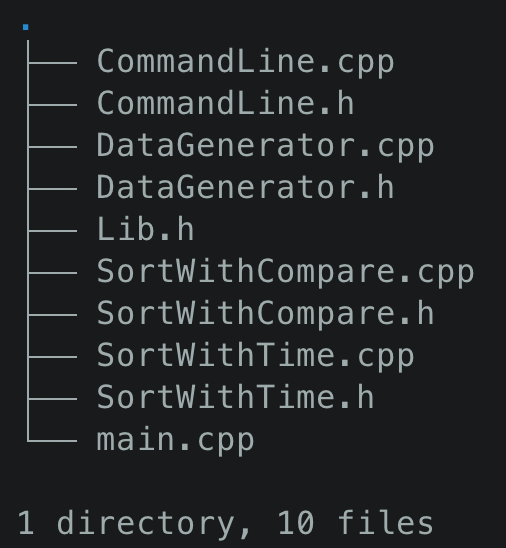
\includegraphics[scale=0.45]{Figures/0. General/tree_folder.png}
    \caption{Folder Tree}
    \label{fig:enter-label}
\end{figure}
% \newpage

% References
% \cleardoublepage
\phantomsection
\bibliographystyle{unsrt}
\bibliography{ref/References}
\cleardoublepage
\phantomsection
\bibliographystyle{unsrt}
\bibliography{ref/References}
\newpage

% % Appendix
% \appendix
% \section{Appendix} 
% \newpage

\end{document}